\documentclass[12pt,a4paper,titlepage]{scrartcl}

\usepackage{preamble}

\title{TP Traitement du signal et problèmes inverses}
\subtitle{Applications sur des exemples EDF}
\author{Saâd Aziz Alaoui, Yassine Jamoud, Samy Haffoudhi}
\date{\today}

\begin{document}

\maketitle

\section*{Introduction}

Lors de ce TP nous allons explorer trois problèmes de traitement
du signal en lien avec des exemples EDF. Le premier problème portera
sur le traitement de signaux multicapteurs illustré sur des données
de température issues de mesures de fibres optiques. Ensuite, nous
nous intéresserons au problème inverse de surrésolution à partir de
données de fibre optique déformation. Enfin, nous verrons le
problème inverse d'estimation des sources à partir de données
de contrôle non destructif ultrasonores.

Pour chacun de ces exemples,
nous commencerons tout d'abord par une présentation du contexte et
de l'enjeu avant de jouer sur les paramètres des différentes méthodes
pour bien appréhender leurs effets.

\section{Traitement de signaux multicapteurs illustré sur des données
de température issues de mesures de fibre optique}

\subsection{Le contexte d'application}

L'objectif de ce premier problème est la détection de fuites dans des digues en terre.
Nous disposons de mesures de températures réparties par une fibre optique
implantée dans la digue. Si il existe une fuite, la température mesurée au niveau de la
fibre optique va subir l'influence de la température de l'eau dans le canal.

On travaille sur les données suivantes :

\begin{figure}[H]
    \caption{Jeu de données}
    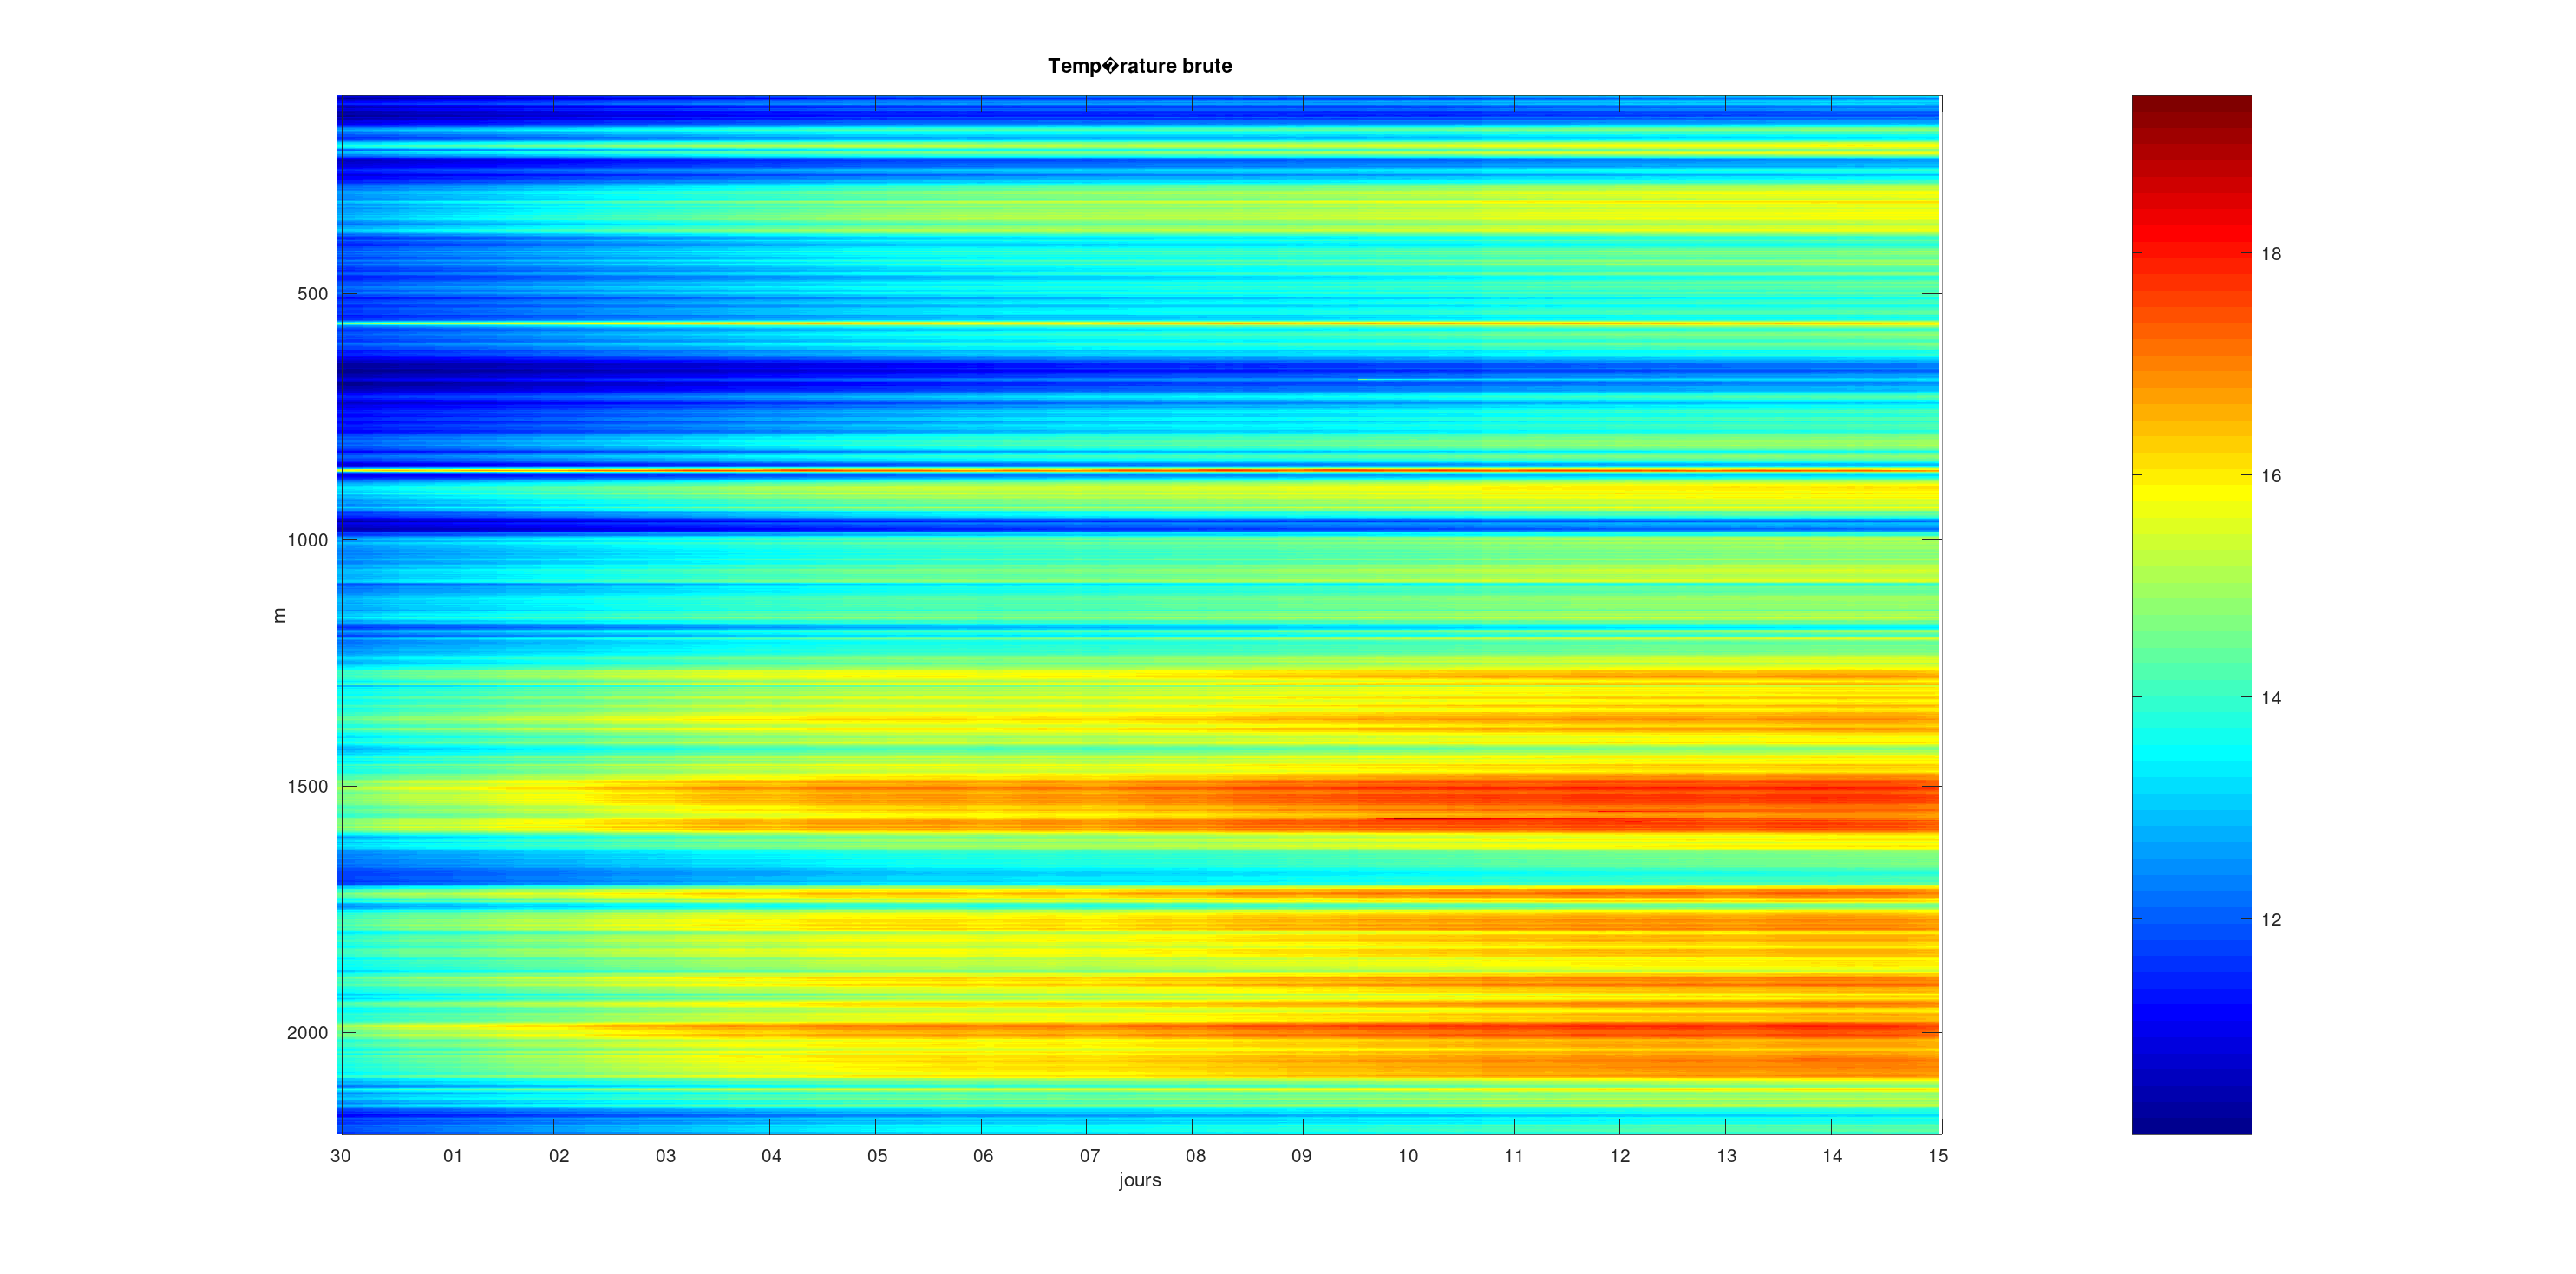
\includegraphics[width=.7\textwidth]{profil}
    \centering
\end{figure}

On centre les températures pour obtenir la figure ci-dessous :

\begin{figure}[H]
    \caption{Jeu de données, températures centrées}
    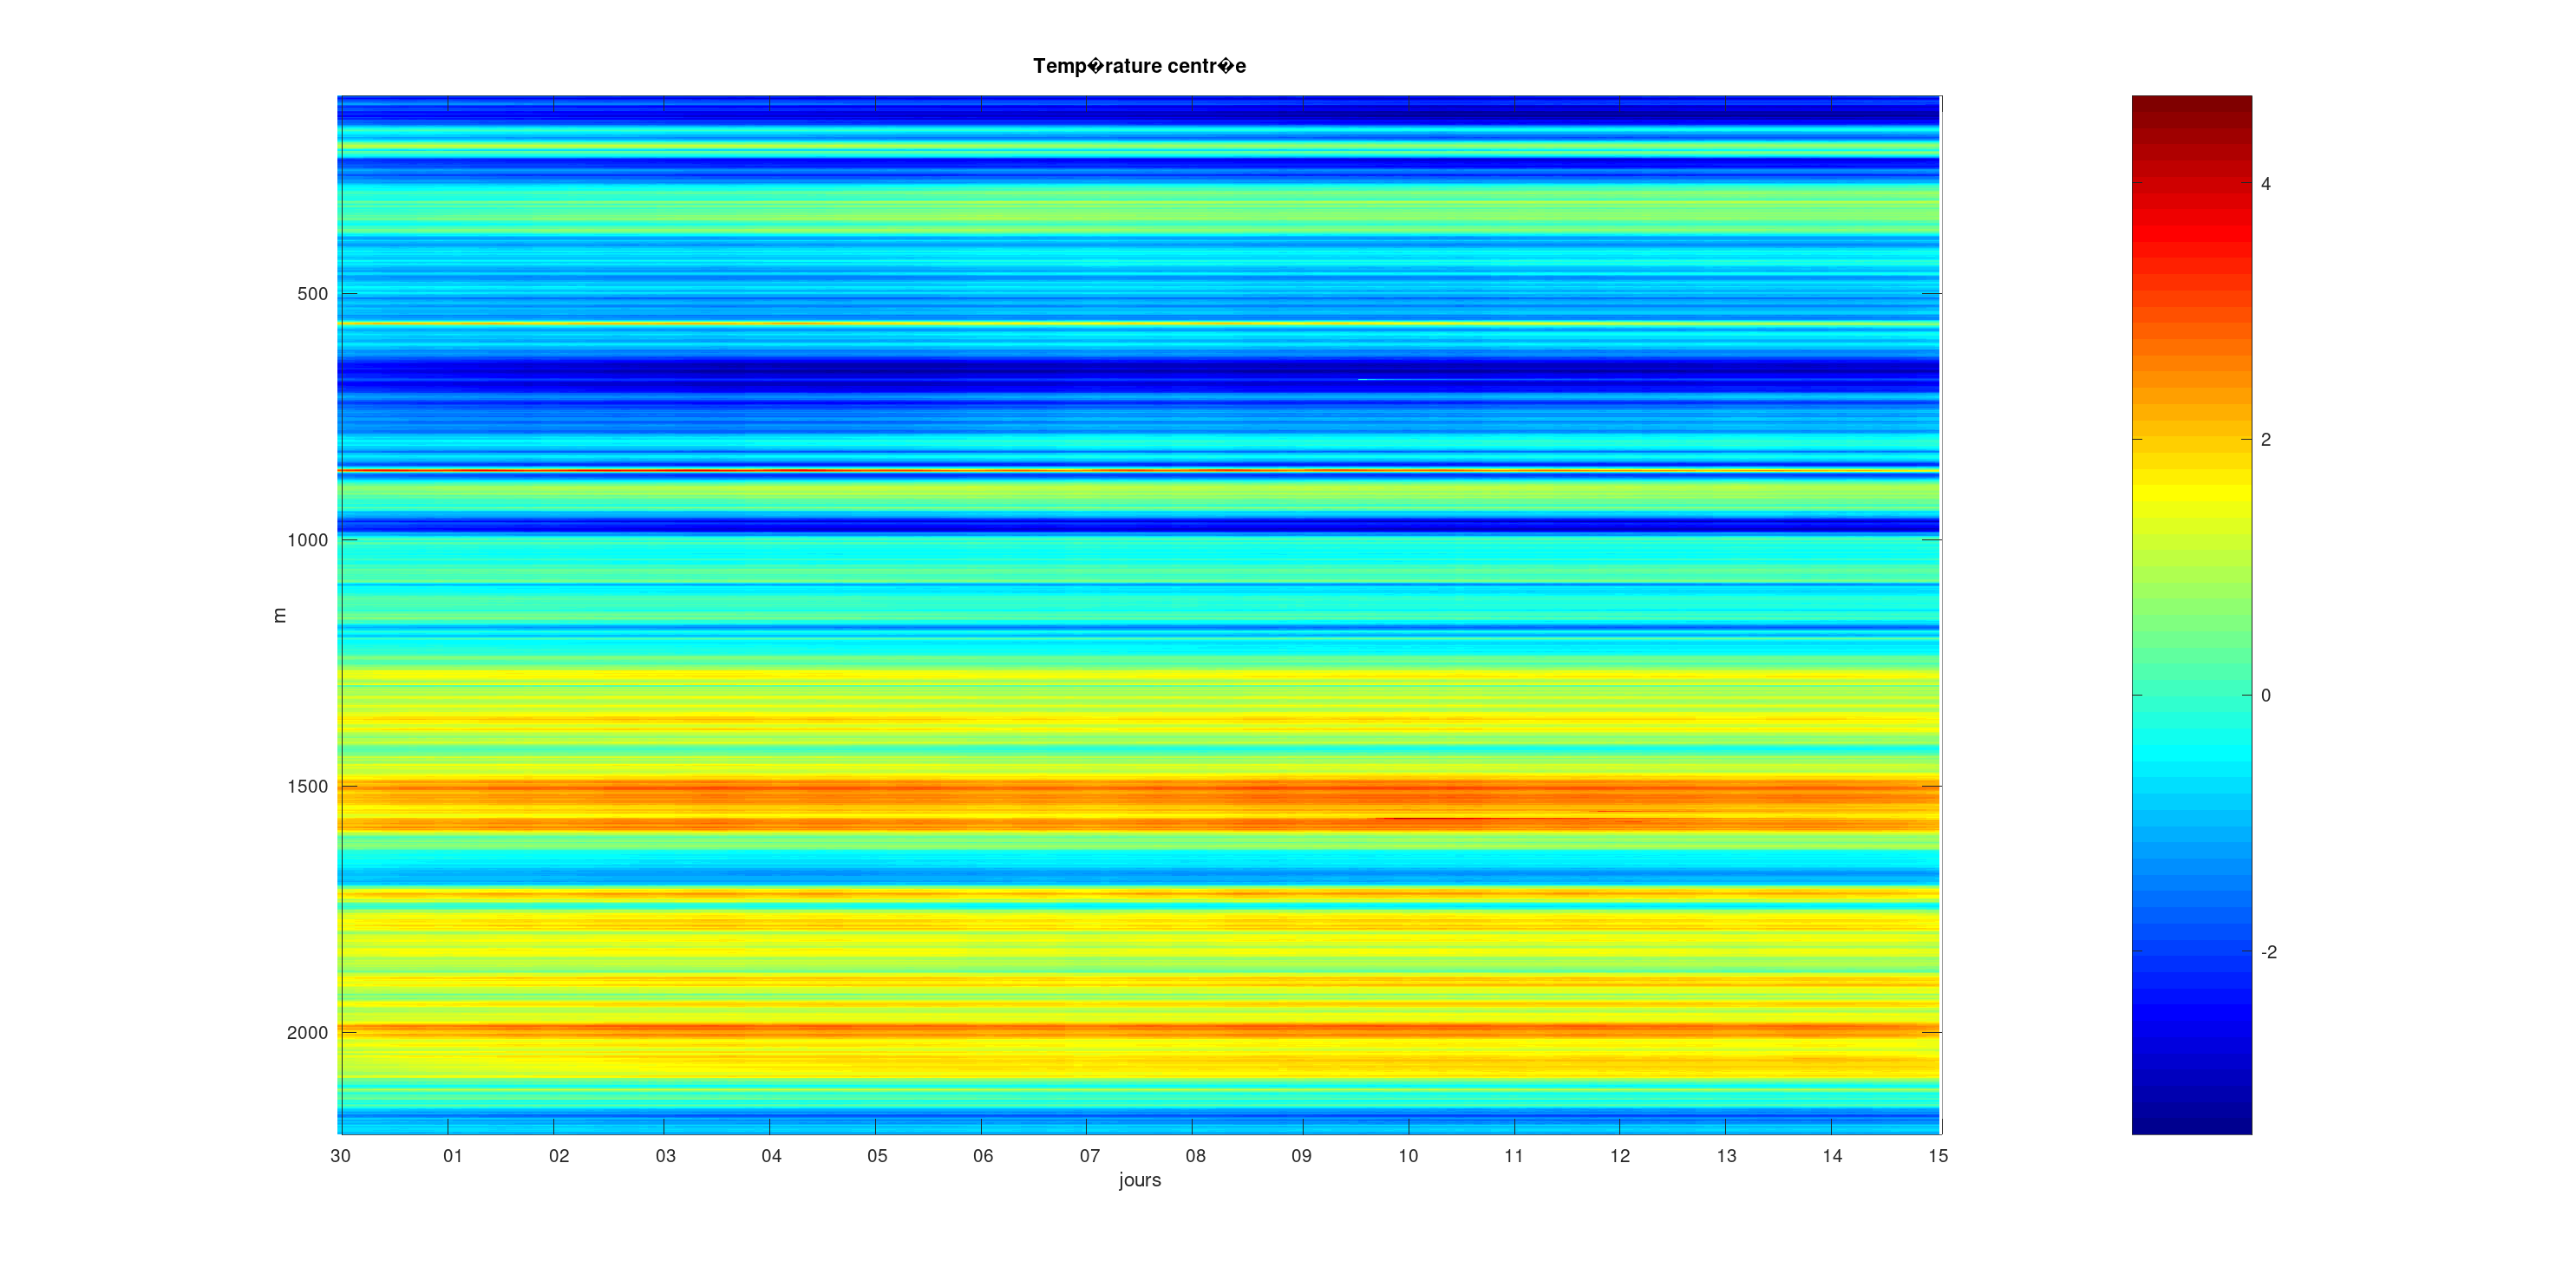
\includegraphics[width=.7\textwidth]{profil_2}
    \centering
\end{figure}

On adopte une approche de séparation de sources, l'objectif étant d'isoler les différentes
sources résponsables des changements de température.

On obtient les valeurs propres suivantes pour l'ACP :

\begin{figure}[H]
    \caption{Valeurs propres ACP}
    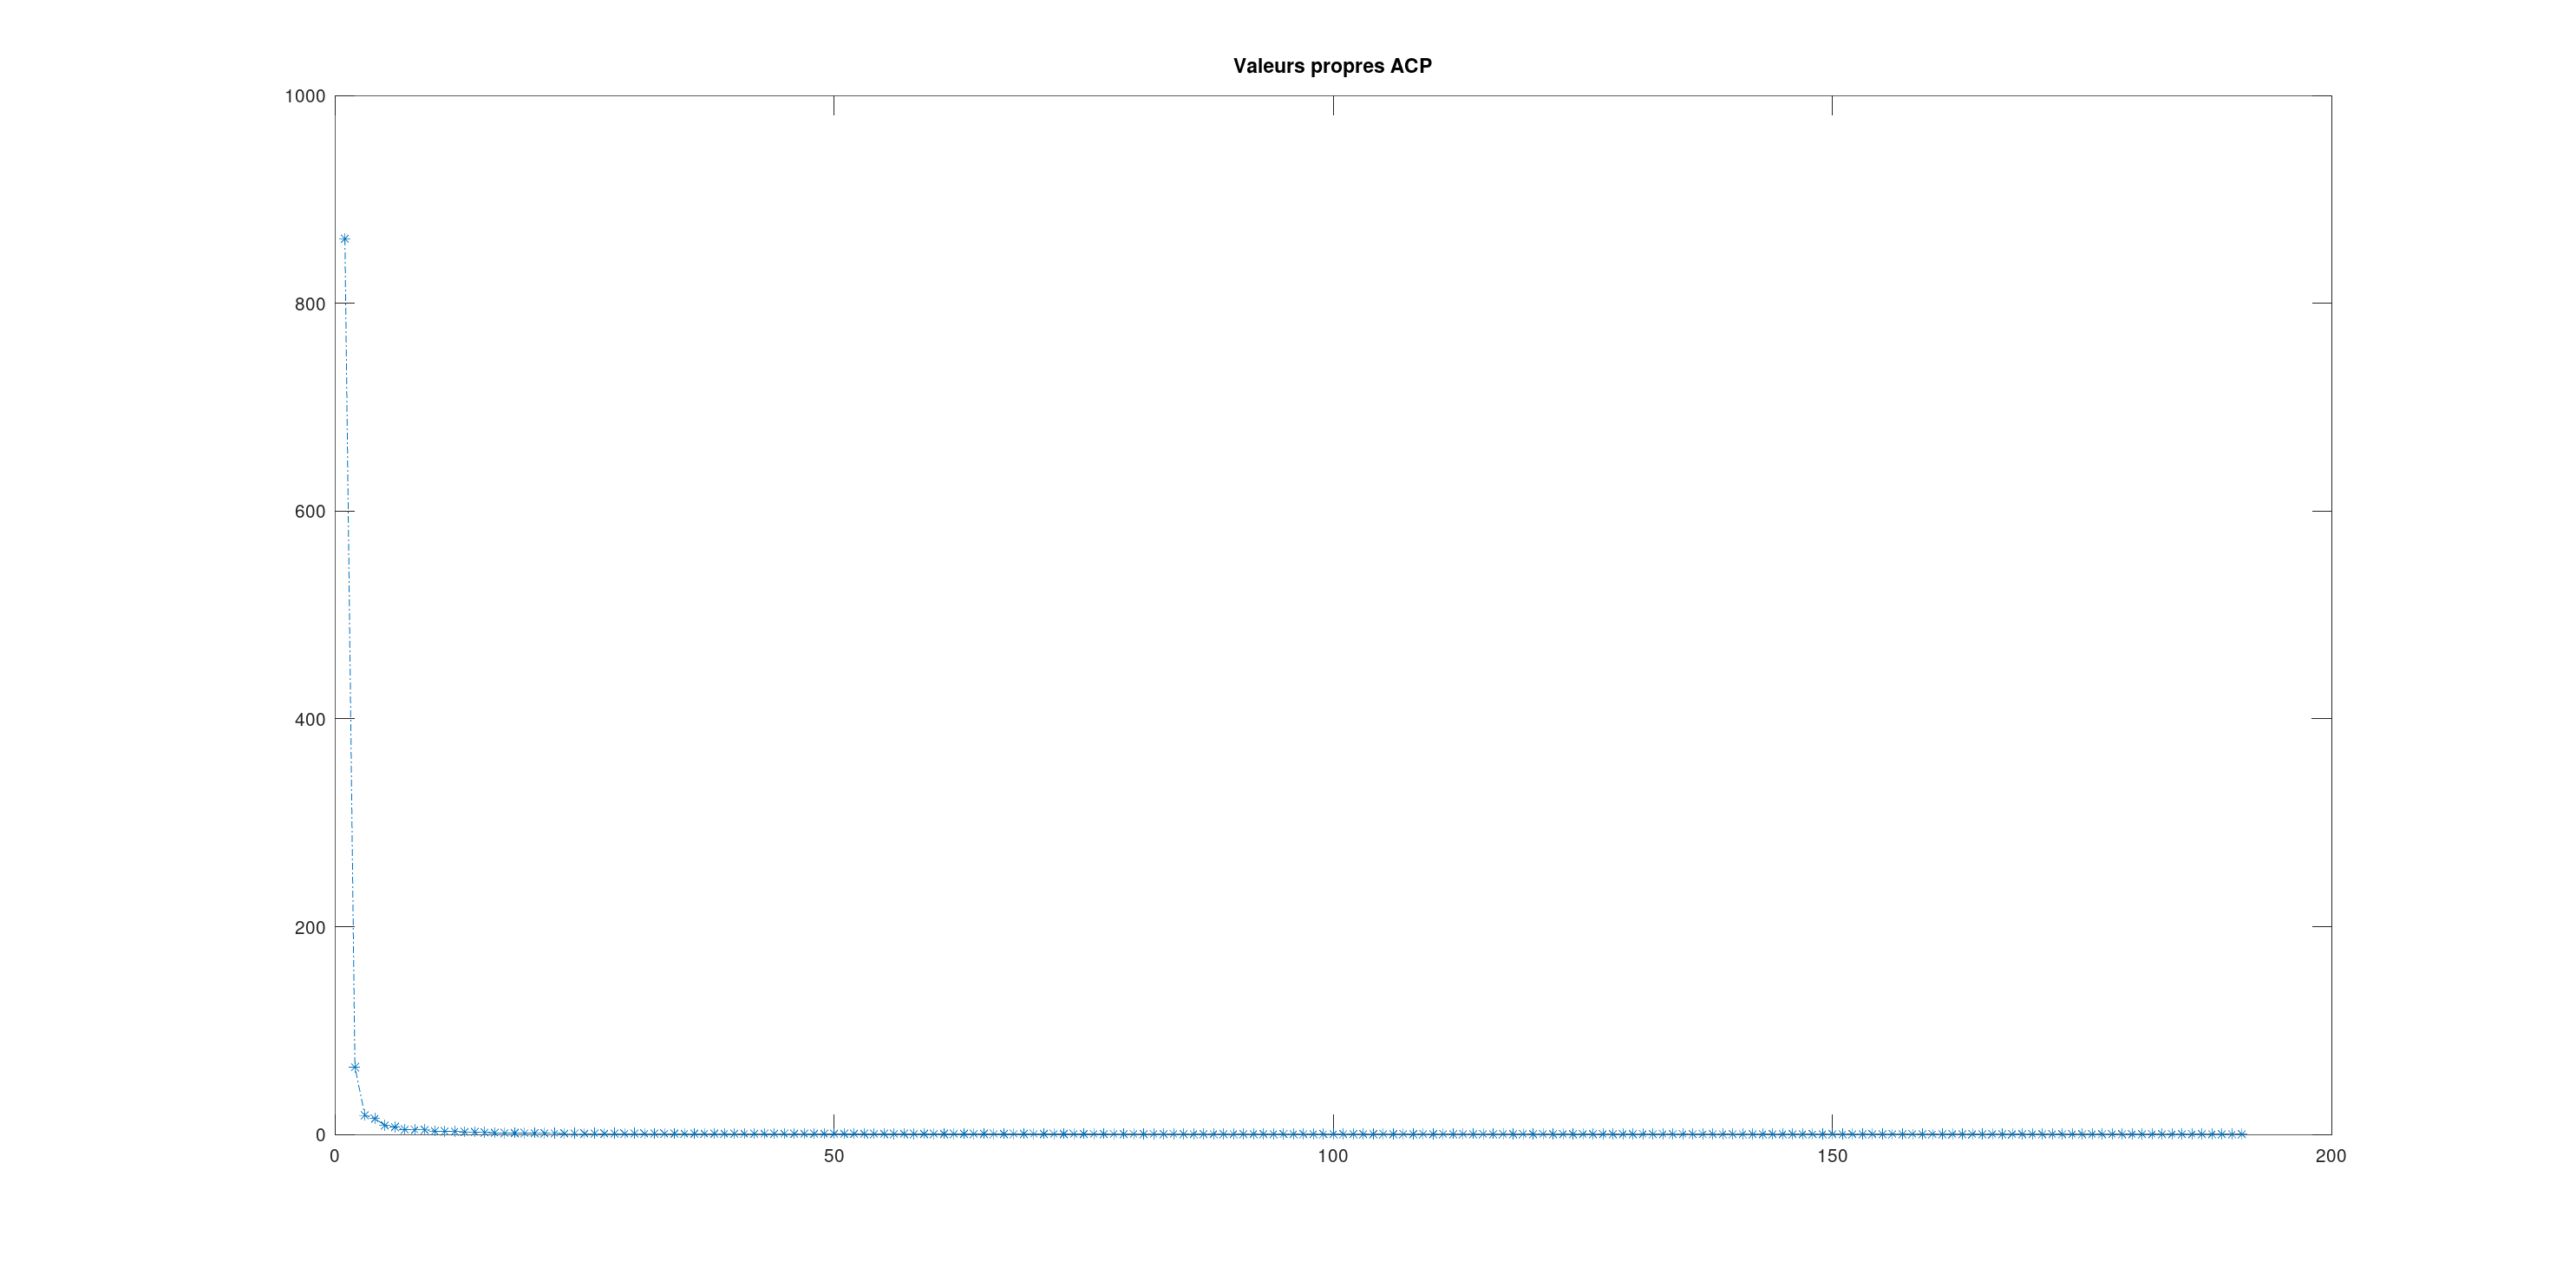
\includegraphics[width=.6\textwidth]{valpropres}
    \centering
\end{figure}

Et affichons les 6 premiers vecteurs propres :

\begin{figure}[H]
    \caption{6 premiers vecteurs propres ACP}
    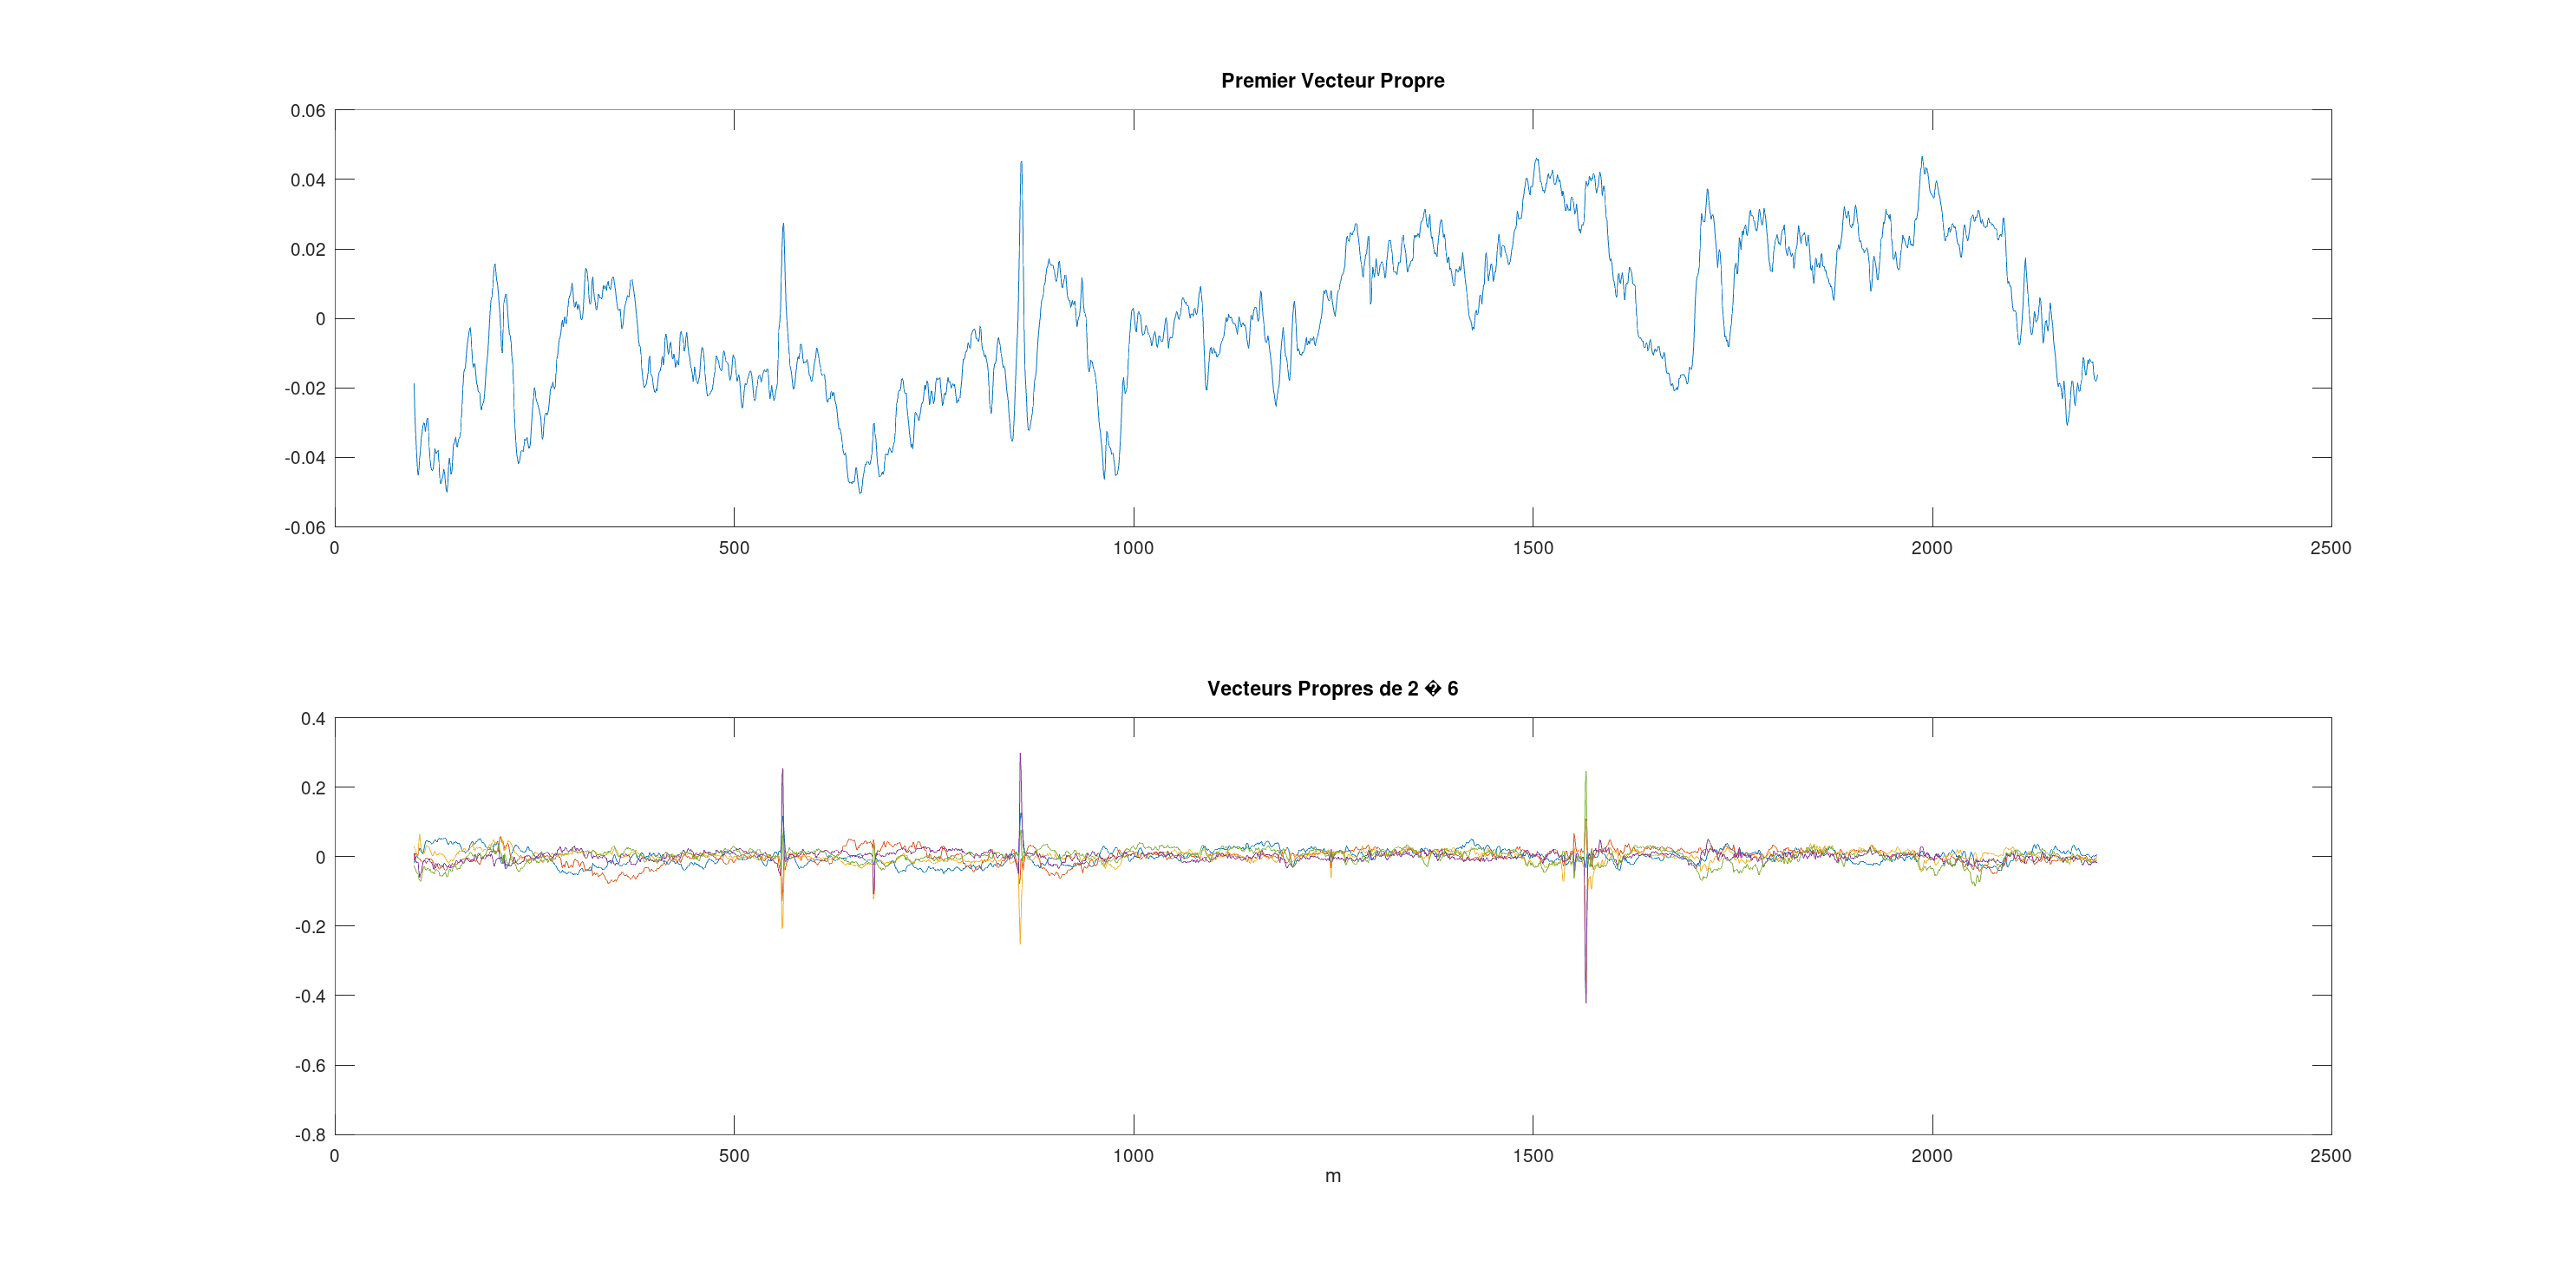
\includegraphics[width=.7\textwidth]{vecteurspropres}
    \centering
\end{figure}

On observe alors que la première valeur propre est bien plus importante que les autres. Elle
correspond à la réponse du sol, on commence alors par supprimer sa contribution.

Après suppression de cette composante, on garde alors les composantes qui correspondent
aux fuites et aux drains. On obtient alors le résidu suivant :

\begin{figure}[H]
    \caption{Résidu ACP}
    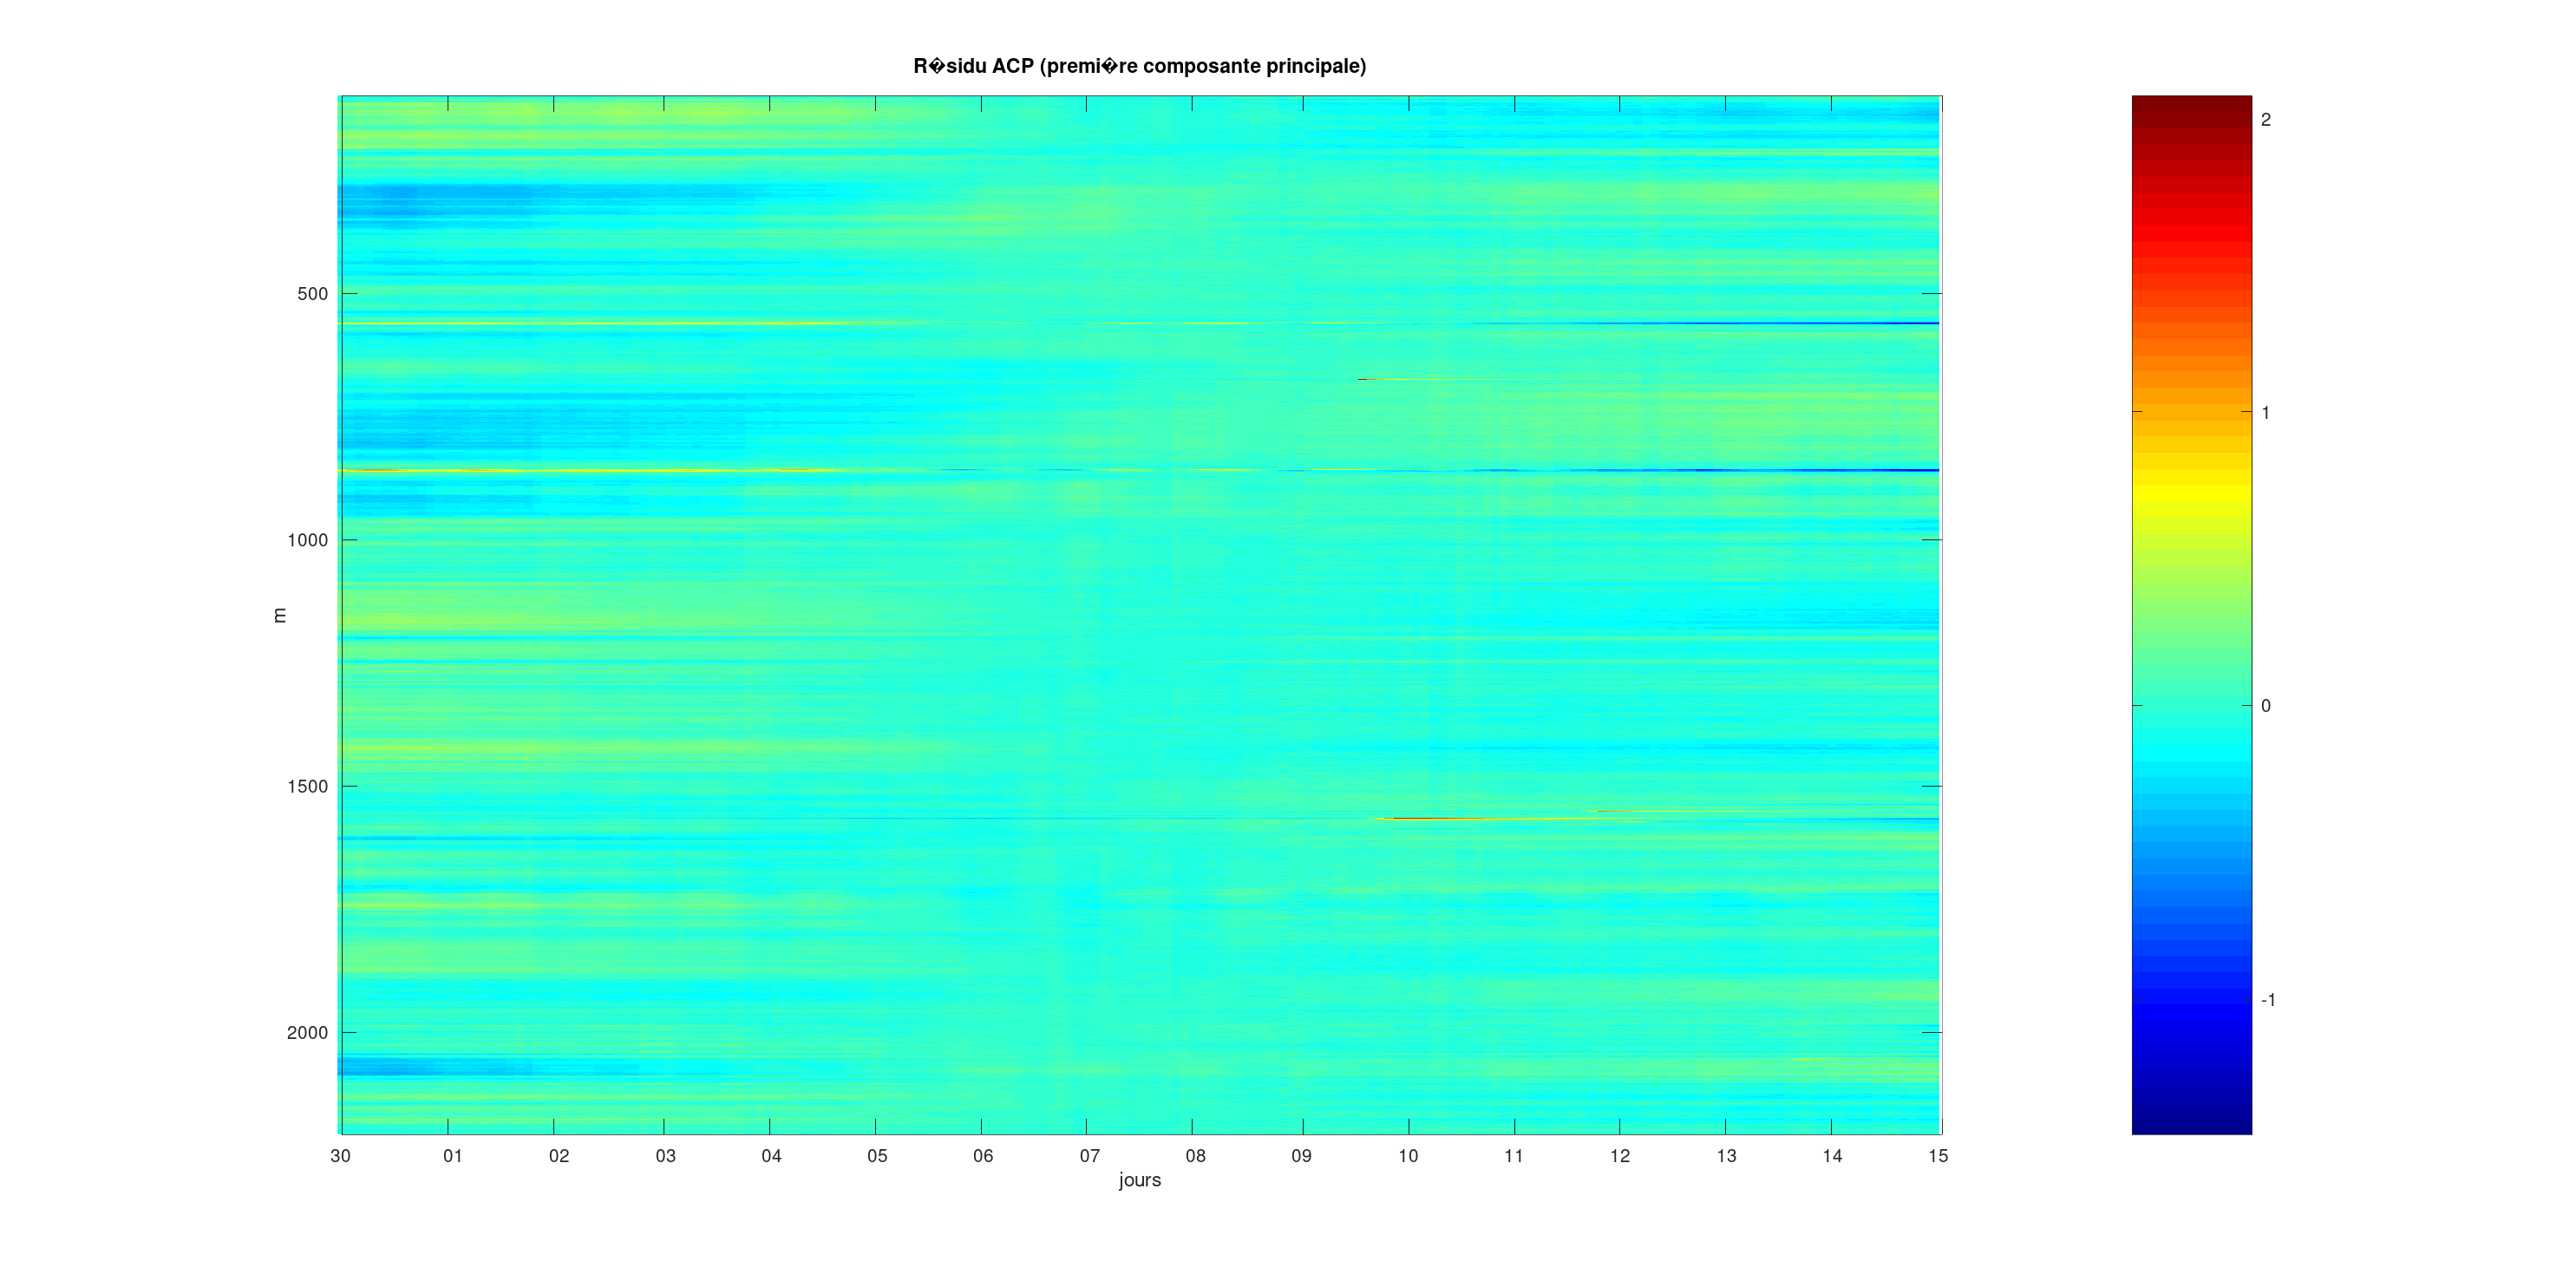
\includegraphics[width=.8\textwidth]{residu}
    \centering
\end{figure}

On obtient déjà une image bien plus claire où l'on peut distinguer uniquement quelques
zones de température élevée. On peut alors détecter l'apparition de la fuite mais, pas
la suivre.

On applique maintenant trois méthodes de séparation de sources : \textbf{Jade}, \textbf{Shibbs} et \textbf{ICA} à partir
d'un nombre de sources donné.

On obtient par exemple pour $N = 4$, les sources suivantes :

\begin{figure}[H]
    \caption{Sources}
    \label{fig:sources4}
    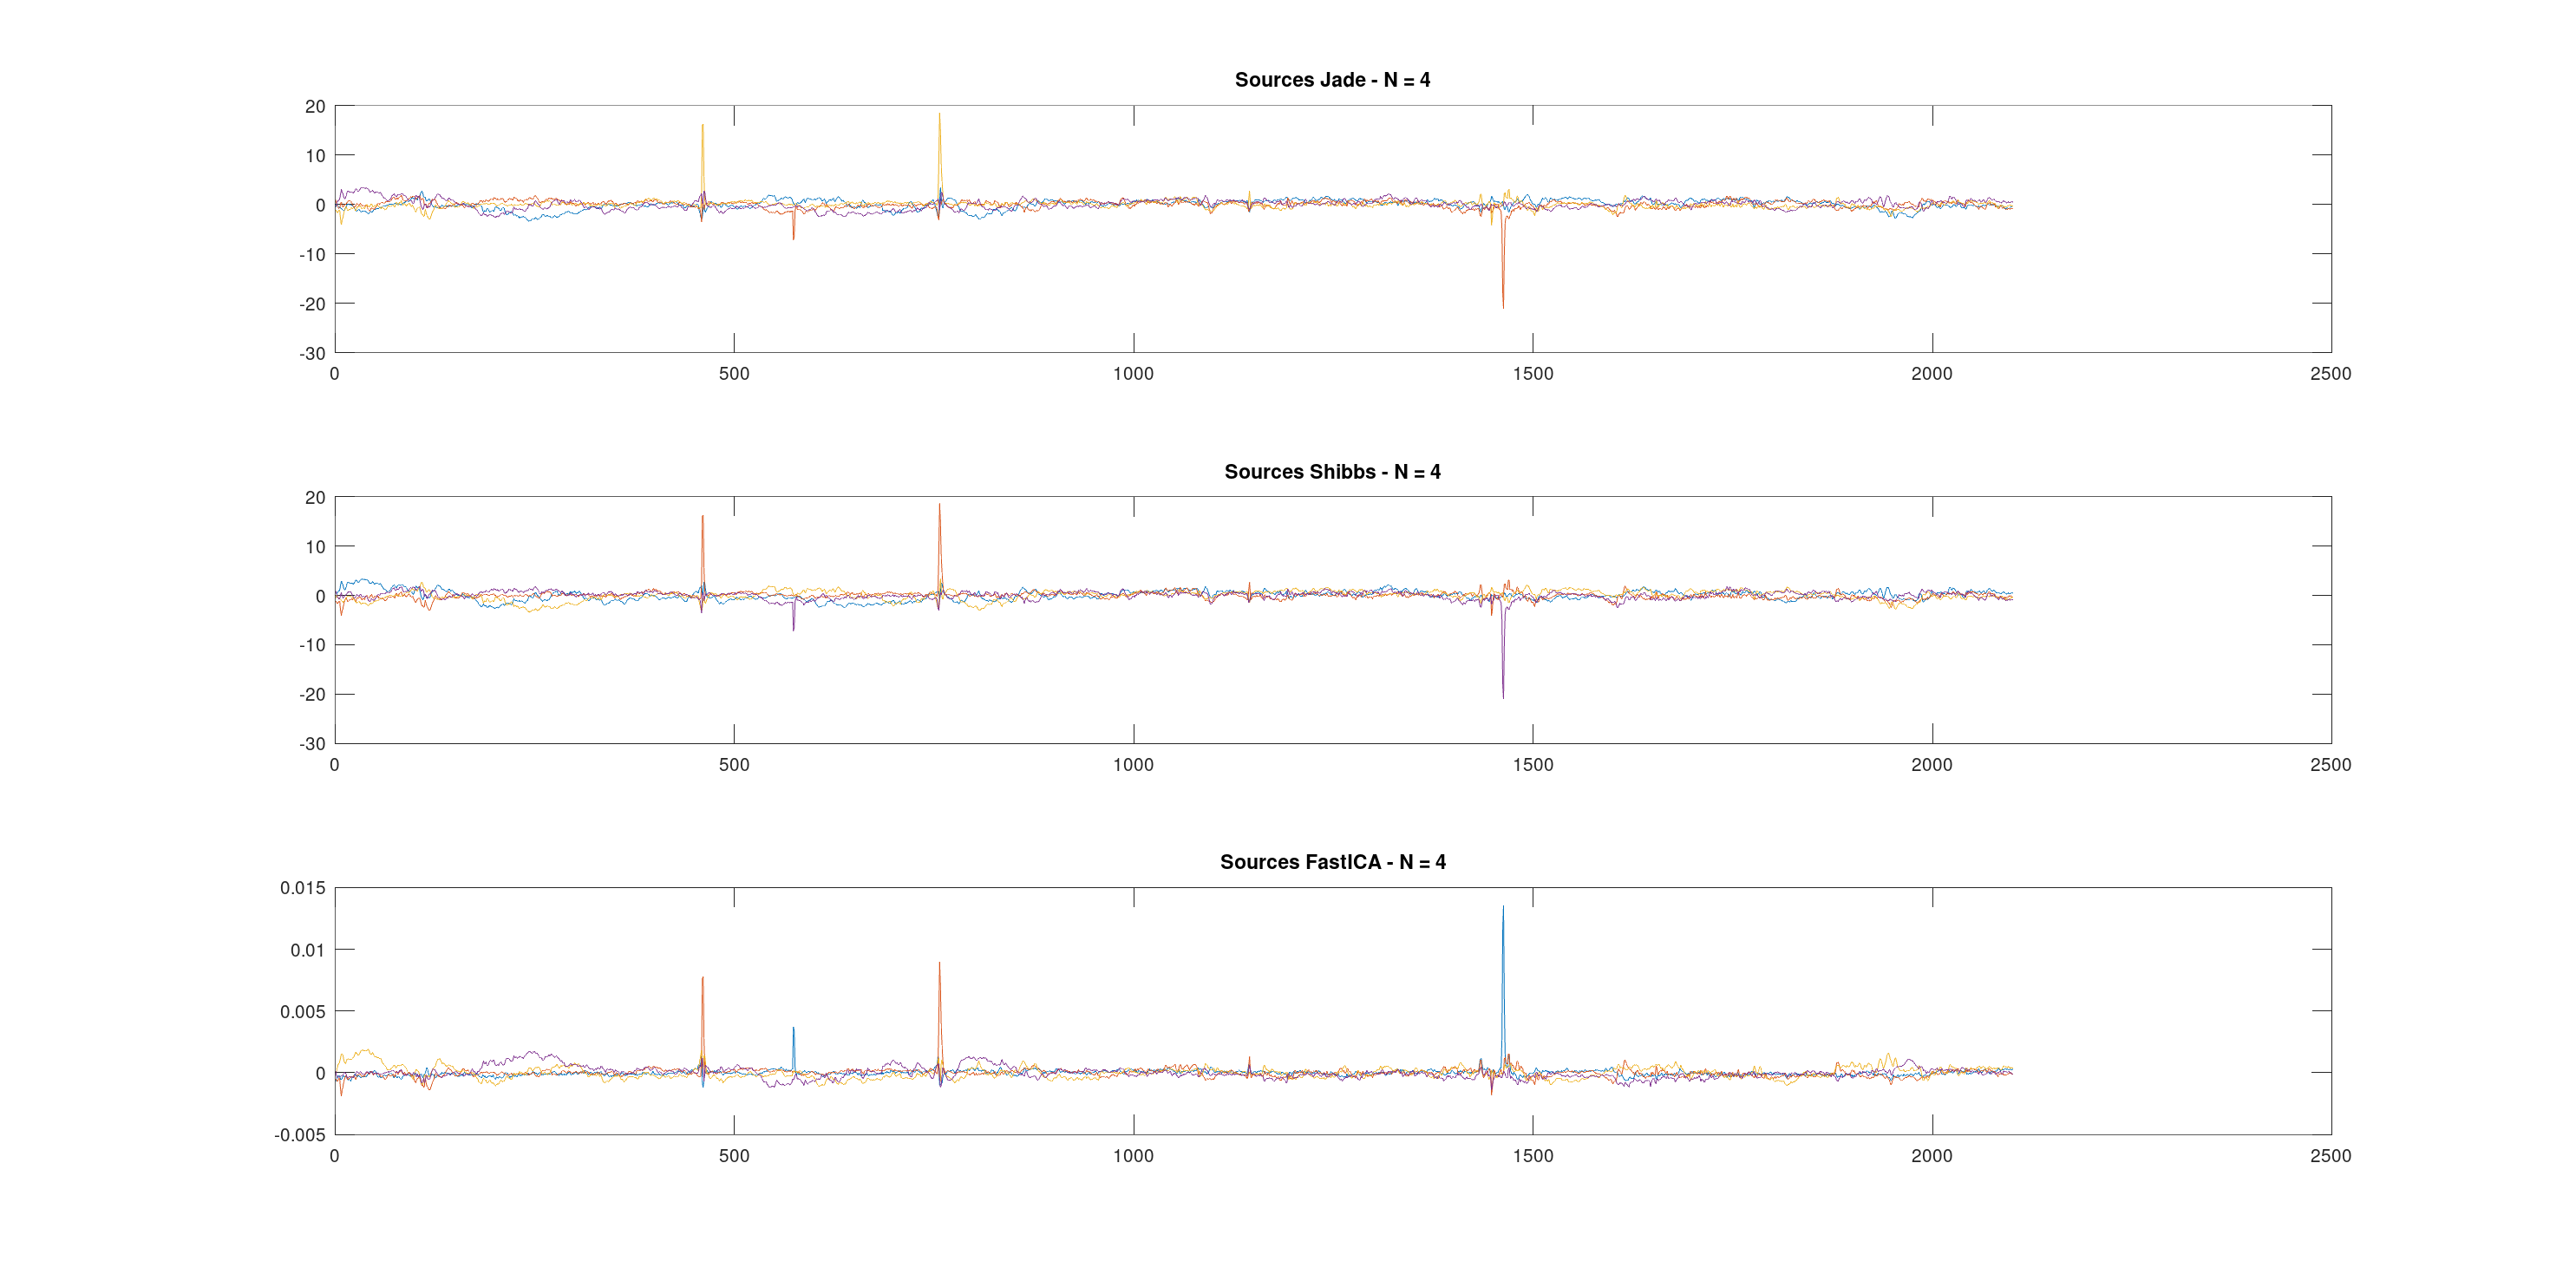
\includegraphics[width=\textwidth]{sources}
    \centering
\end{figure}

Et ces résidus :

\begin{figure}[H]
    \caption{Résidus}
    \includegraphics[width=\textwidth]{résidus}
    \centering
\end{figure}

\subsection{Influence des paramètres}

Le paramètre sur lequel nous pouvons jouer pour ce problème est le nombre
de sources pour les différentes méthodes. Nous avons tracé les figures ci-dessus
avec une valeur de 4 pour ce paramètre.

Considérons maintenant  le cas d'un nombre de sources égal à 1.

On obtient la figure suivante pour les sources :

\begin{figure}[H]
    \caption{Sources}
    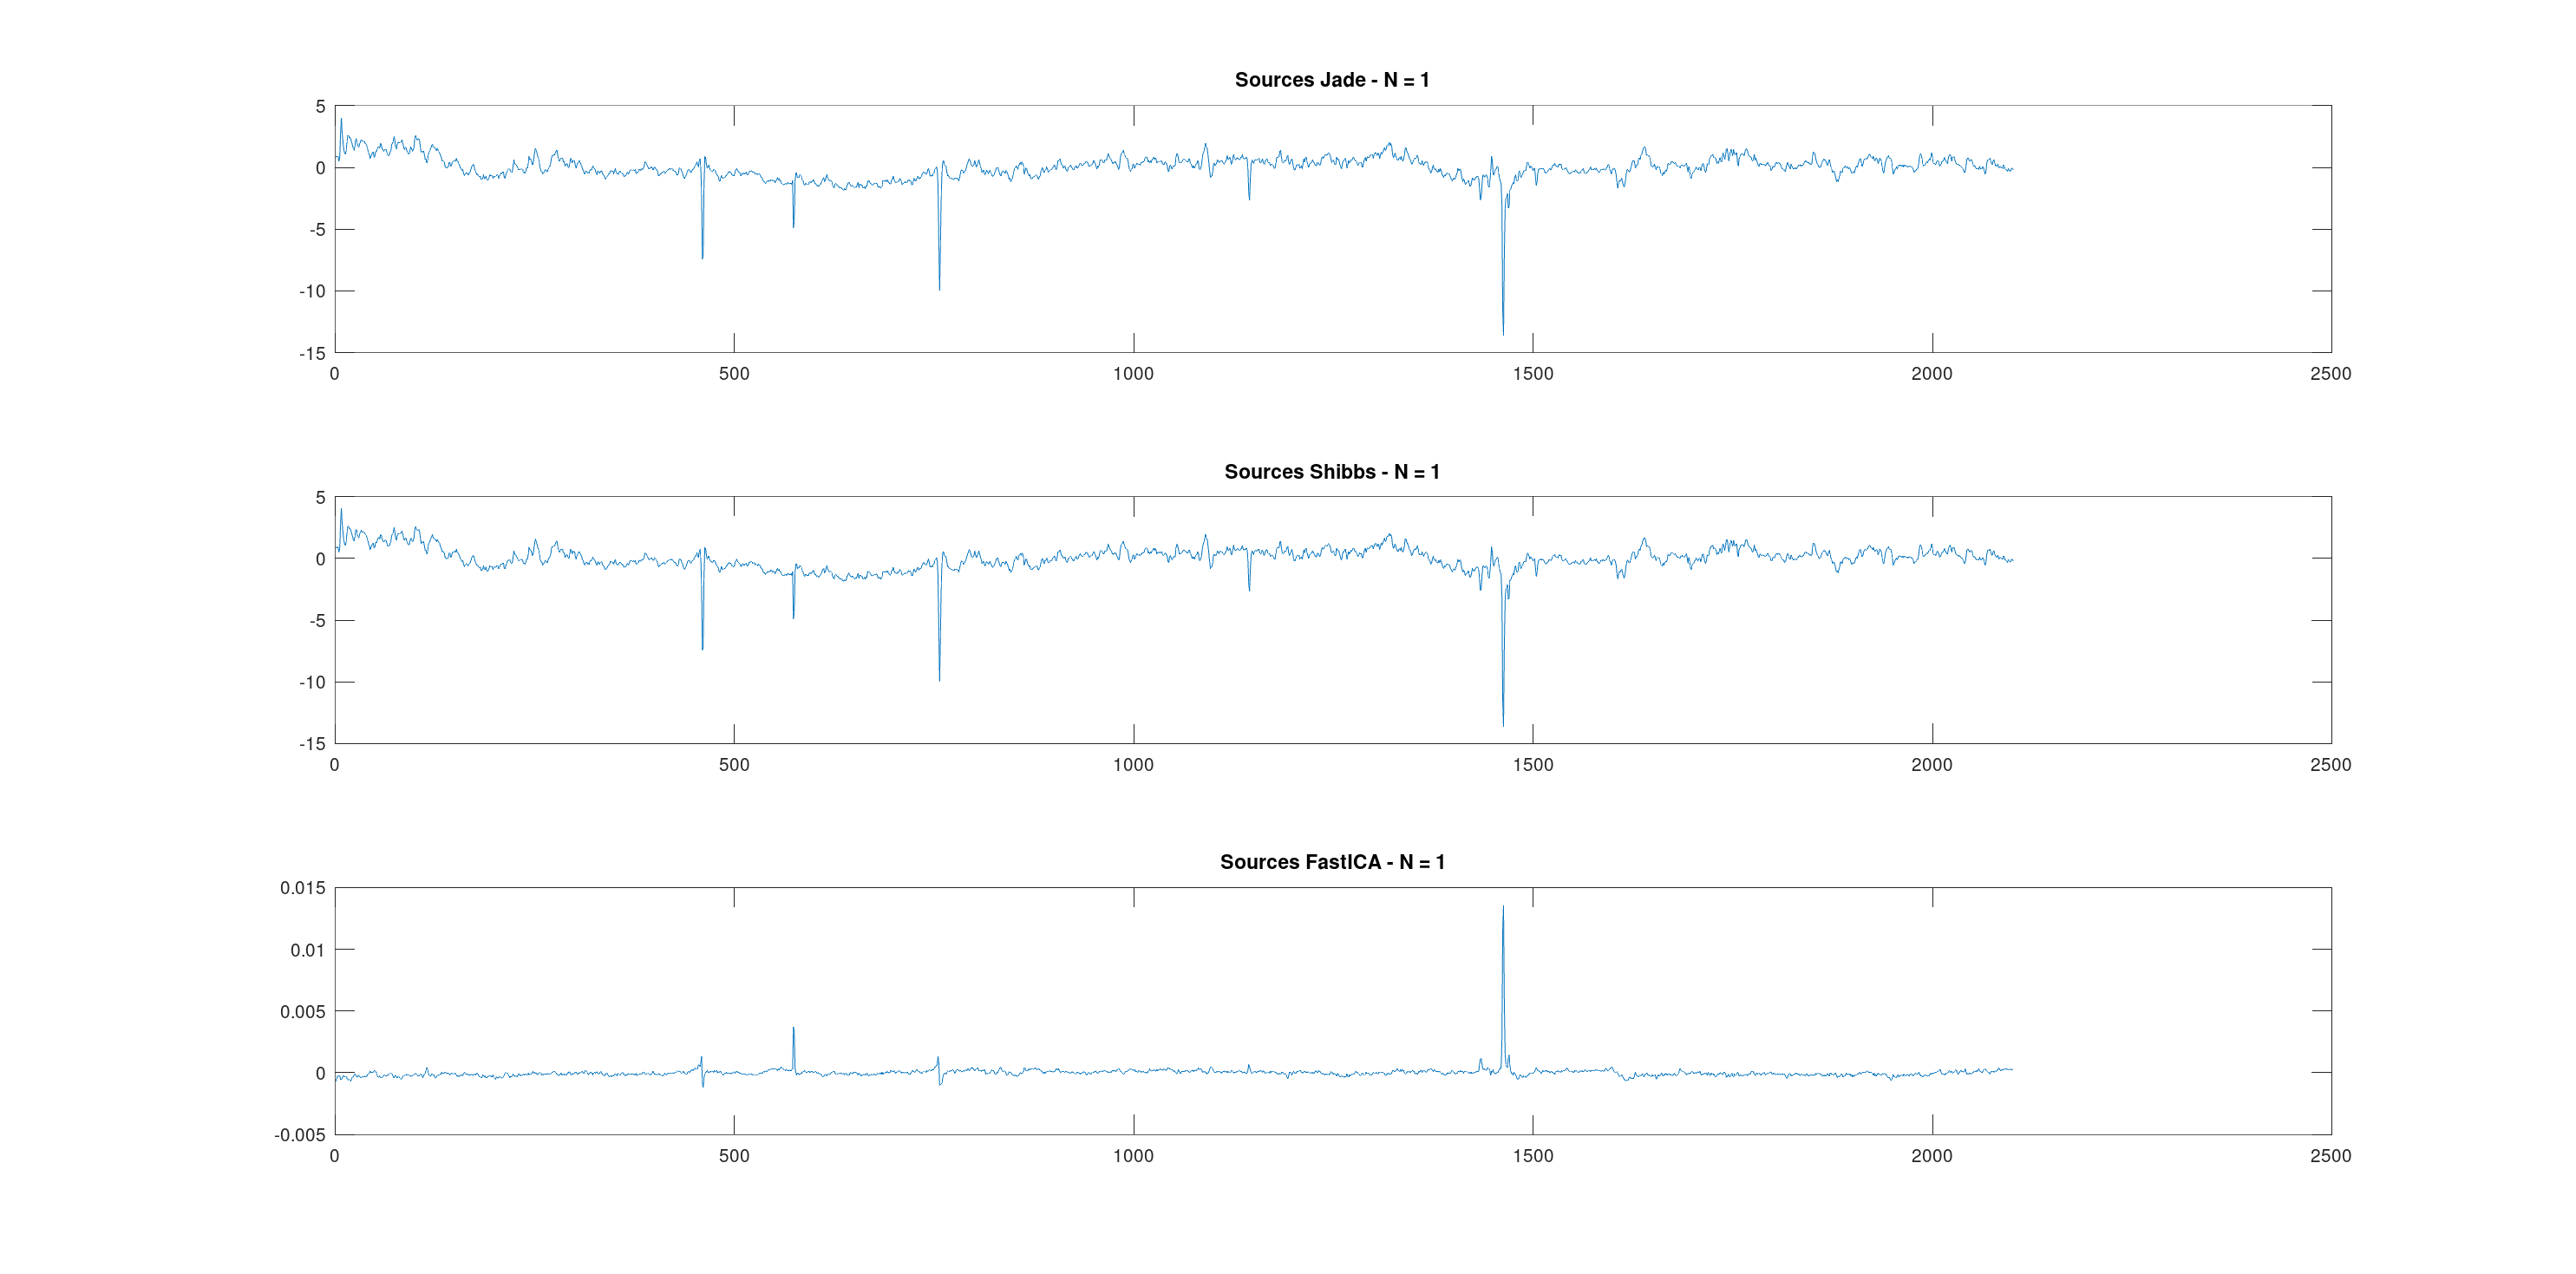
\includegraphics[width=\textwidth]{sources_2}
    \centering
\end{figure}

Et pour les résidus :

\begin{figure}[H]
    \caption{Résidus}
    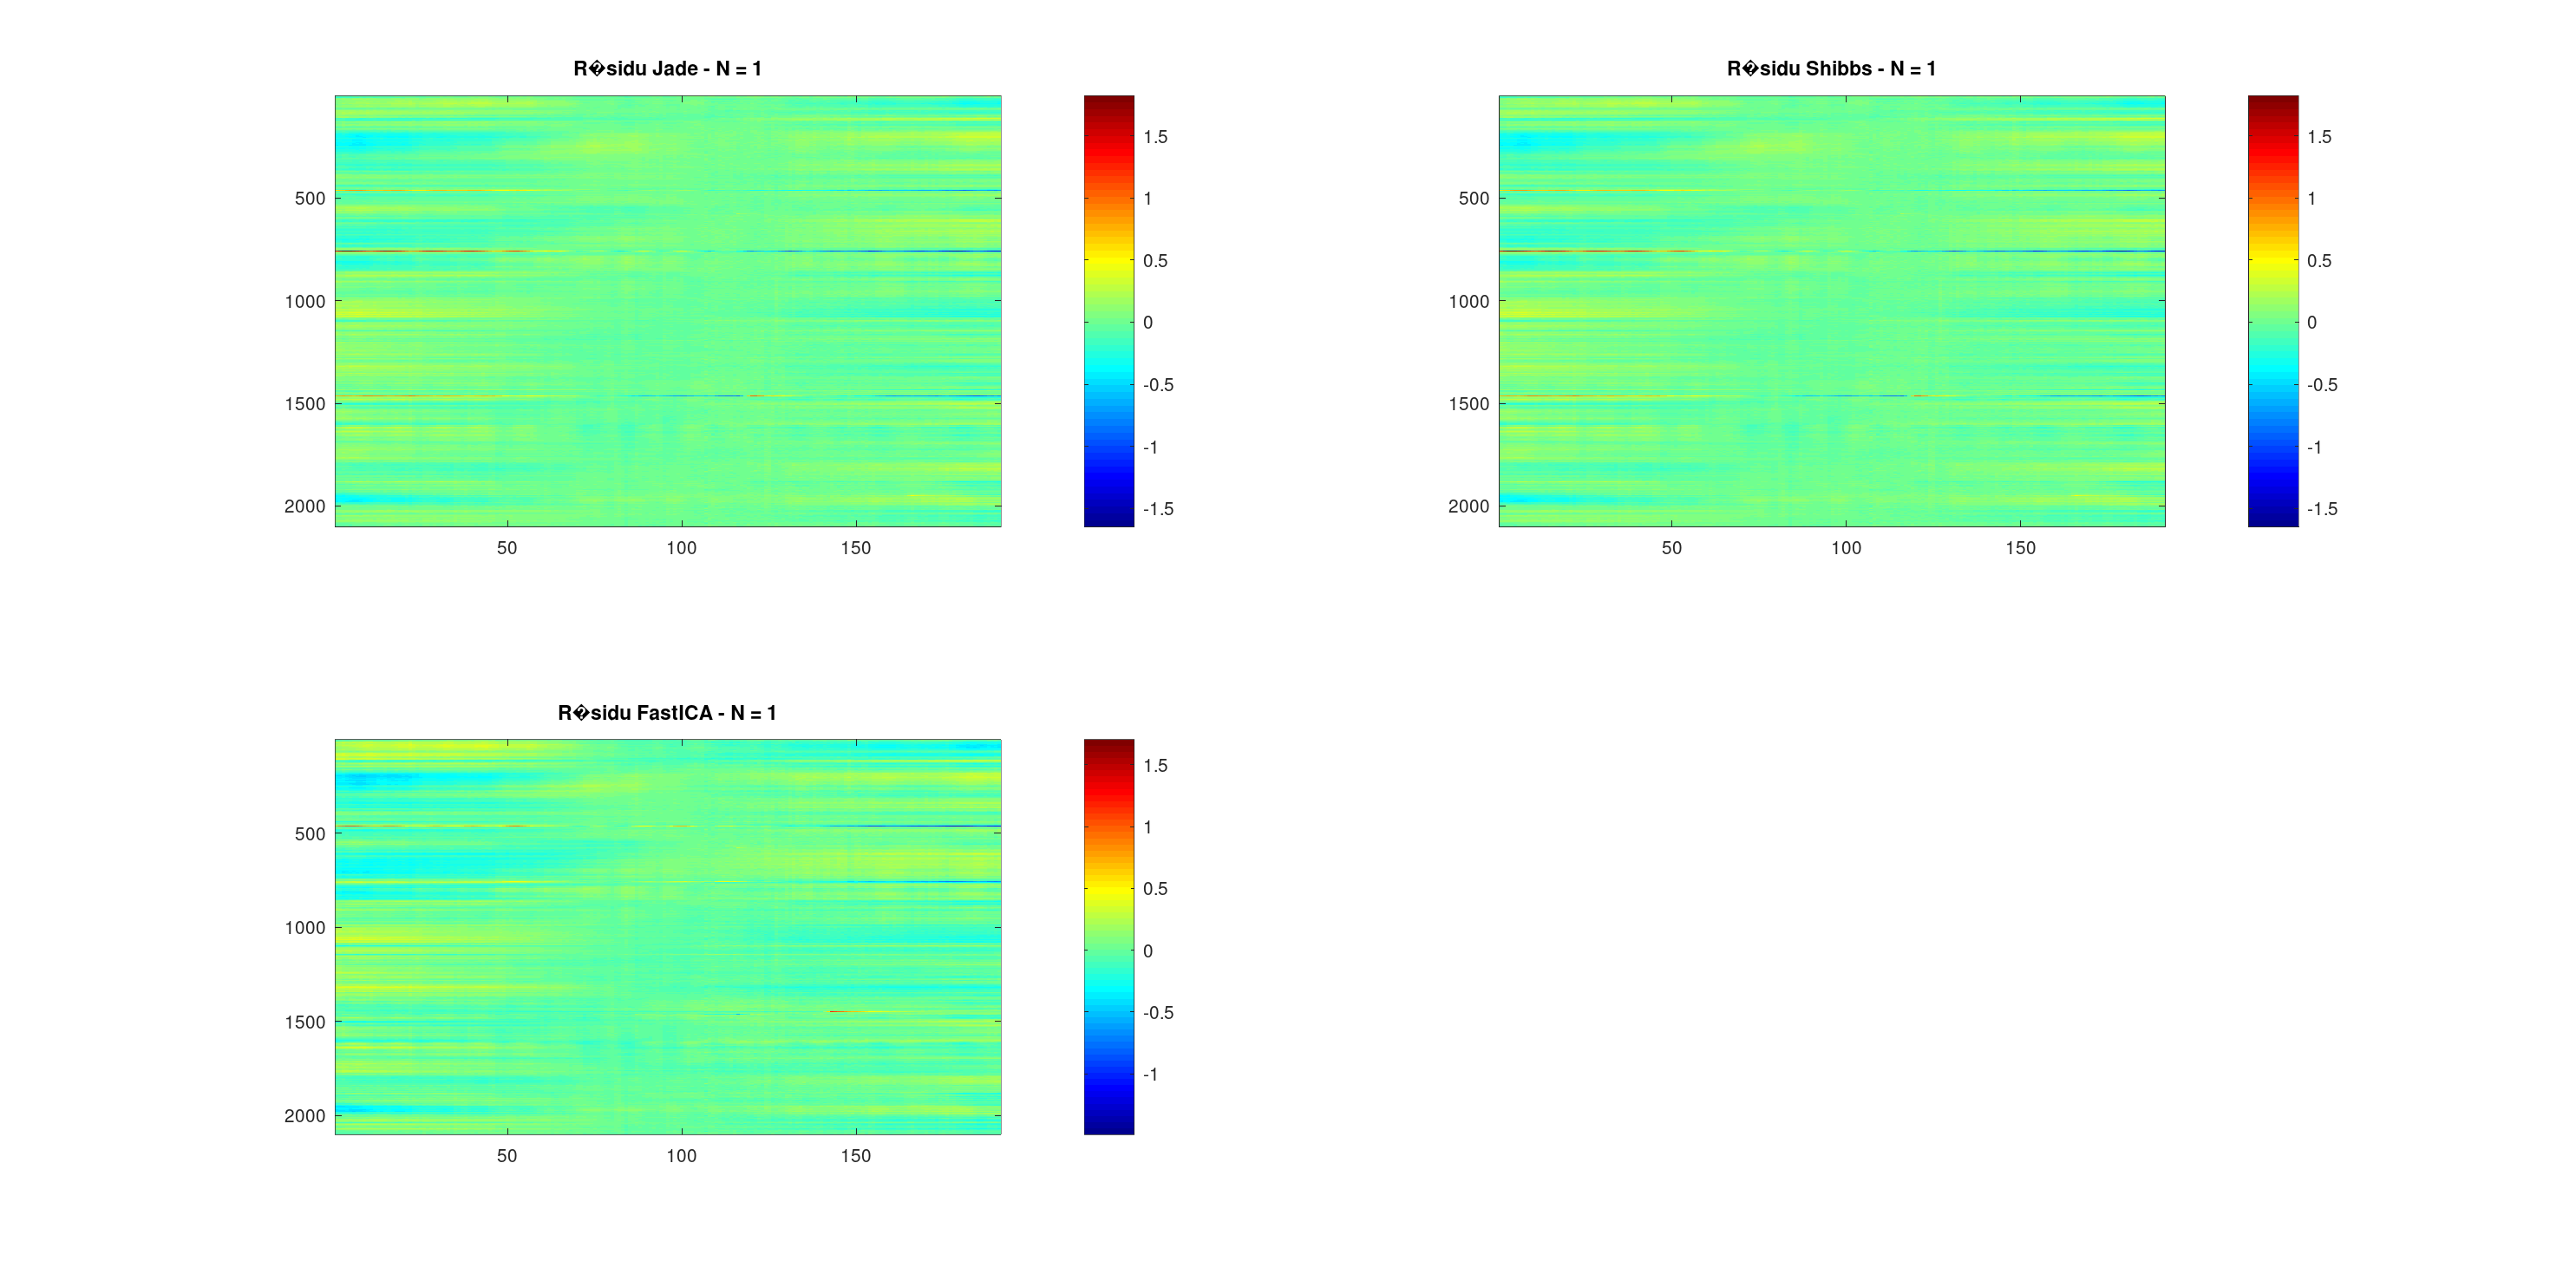
\includegraphics[width=.9\textwidth]{residus_2}
    \centering
\end{figure}

On observe alors sur ces figures que la méthode ICA résulte en moins de bruit que les
deux autres méthodes. Le bruit est par exemple induit par des restes de la contribution
du sol ou le drainage. Pour les deux premières méthodes qui prennent encore en compte ce
bruit, on regarde alors les résidus. Le paramètre et la méthode utilisés indiquent alors si
il faut plutôt observer les sources ou le résidu pour identifier les fuites.

\pagebreak

\section{Problème inverse de surrésolution à partir de données de fibre optique déformation}

\subsection{Le contexte d'application}

L'objectif de ce second problème est la localisation de fontis dans des digues en terre ou
de déformations locales dans des bâtiments. Nous disposons de mesures de spectres par fibre
optique pour estimer les déformations. Le but est alors de passer d'une information intégrée
à une information plus locale. On va alors chercher à estimer à partir de mesures de spectre
sur un intervalle, des spectres locaux.

Voici les données brutes :

\begin{figure}[H]
    \caption{Données brutes}
    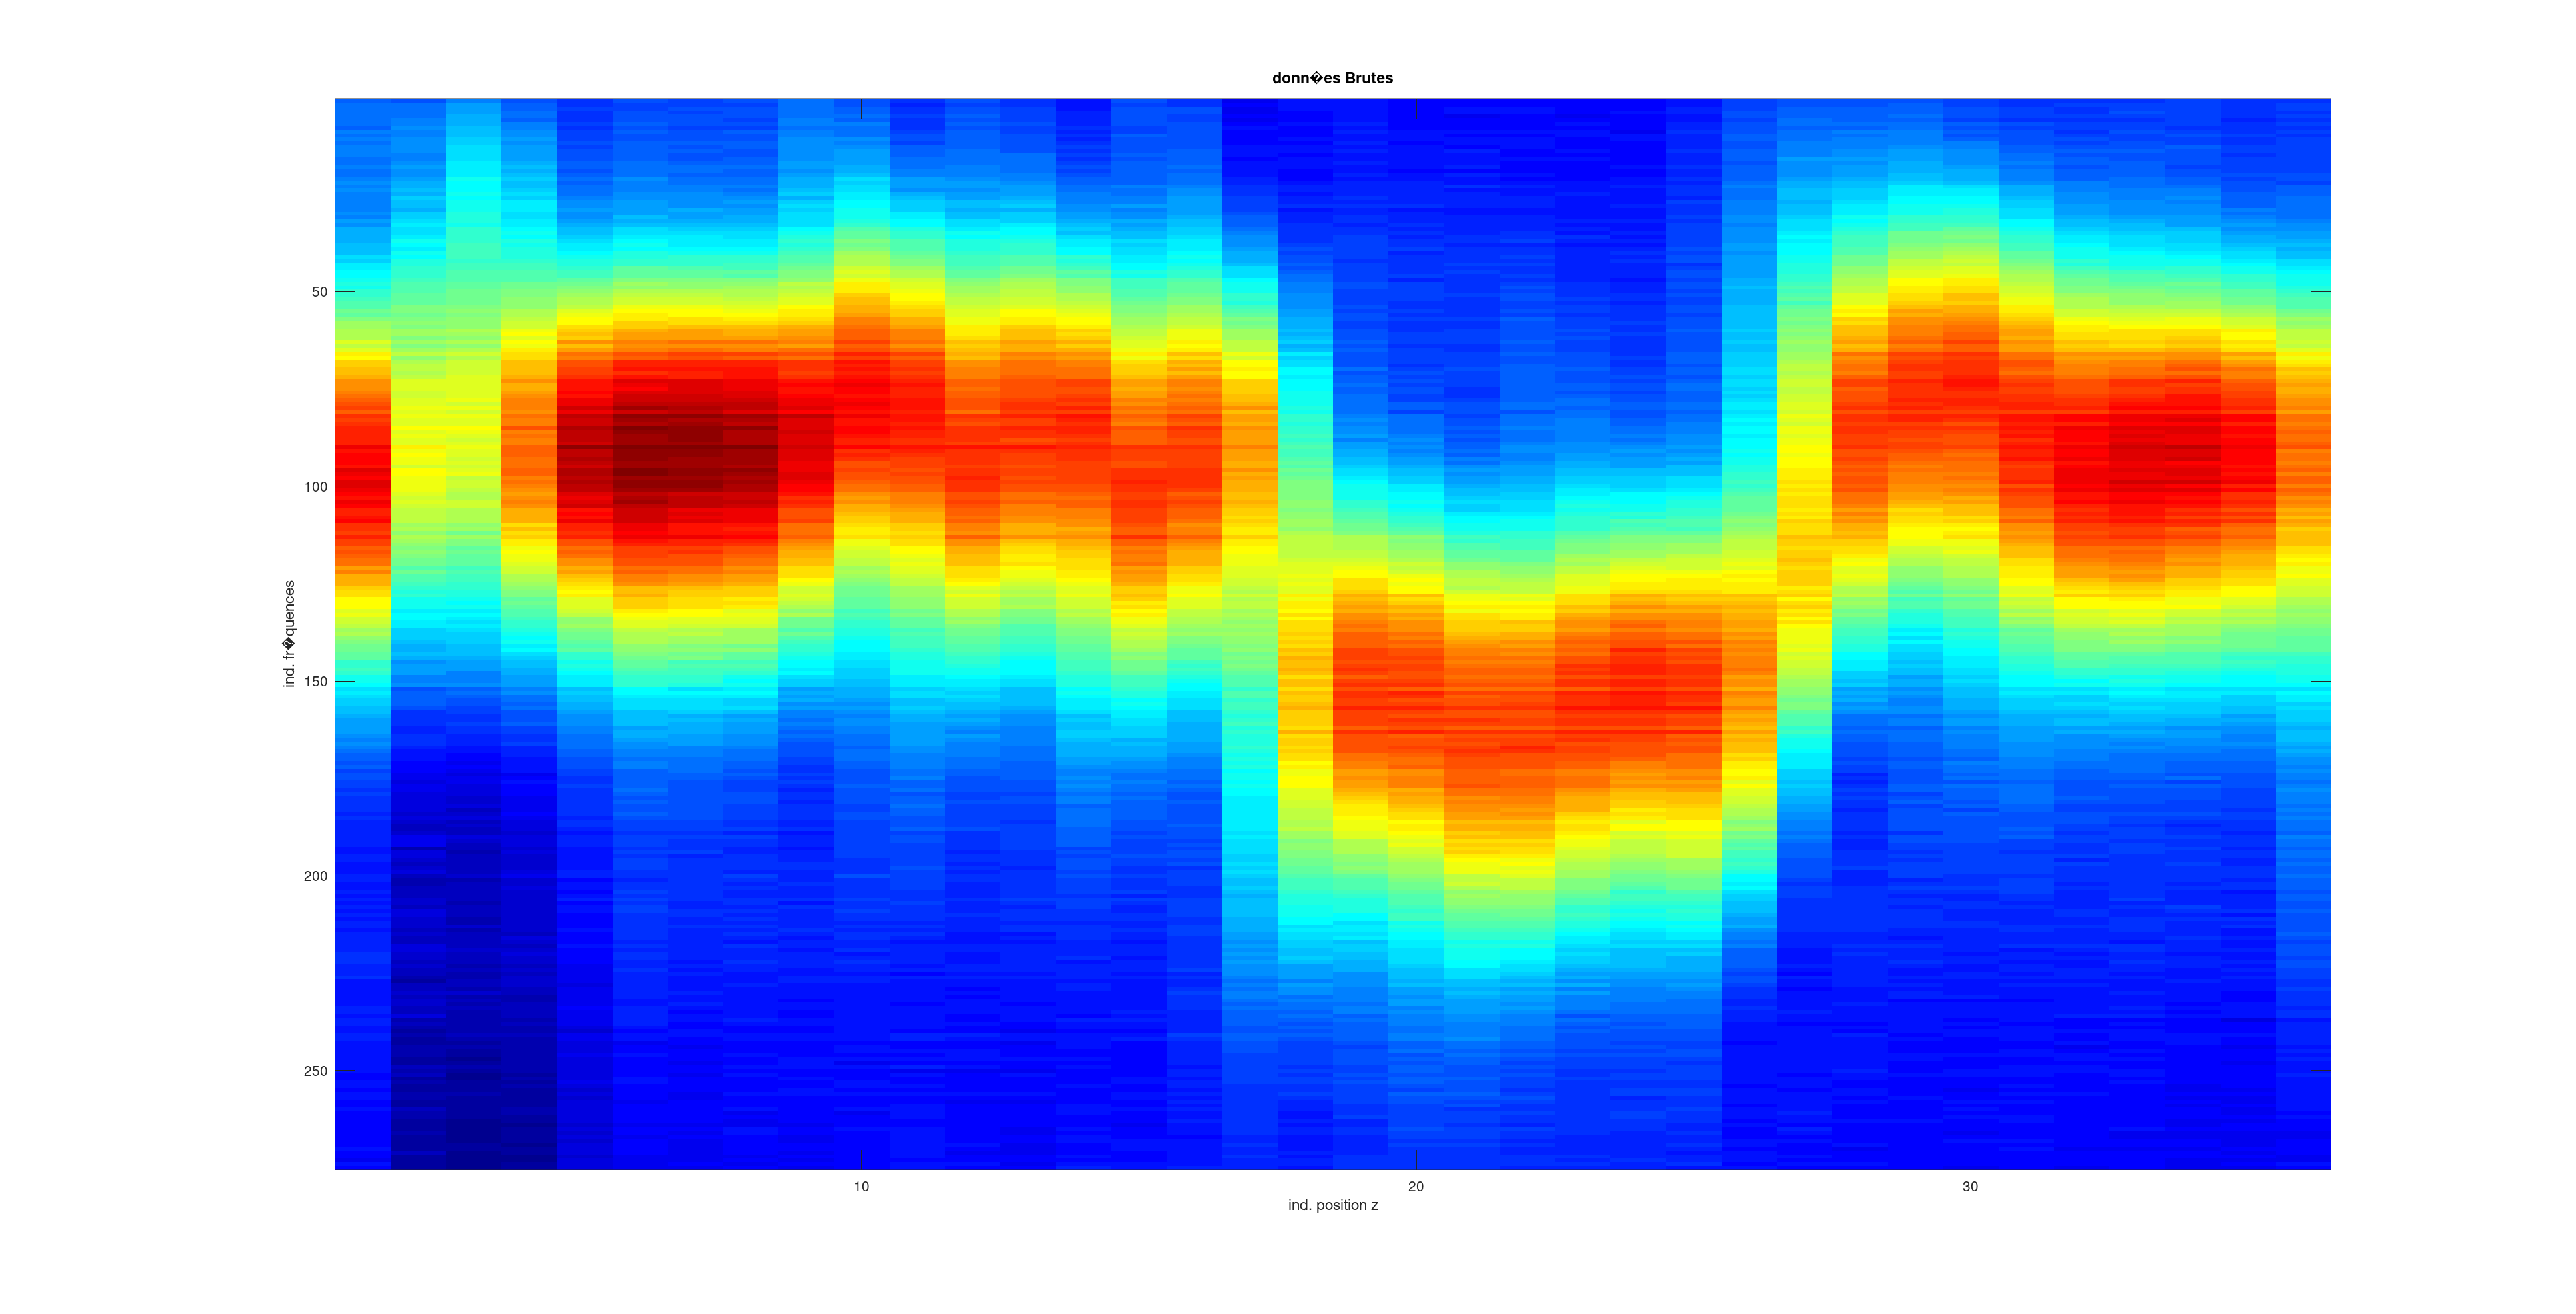
\includegraphics[width=.8\textwidth]{spectreint}
    \centering
\end{figure}

Cette figure indique alors une déformation aux alentours de $z = 16$. Mais ce spectre n'est
pas assez précis. En effet, on observe clairement un étalement en $z$.

Il s'agit d'un problème de déconvolution :

$$ G(\nu, z) = W_z *_x s(\nu,x) $$

On cherche $s$ mesurant $G$ avec $W_x$ un opérateur de moyenne.

Une première approche consiste alors en la résolution du problème d'optimisation

$\min \lVert x \rVert^2$ sous la contrainte $y = Hx$.

On obtient le résultat suivant :

\begin{figure}[H]
    \caption{Rétropropagation}
    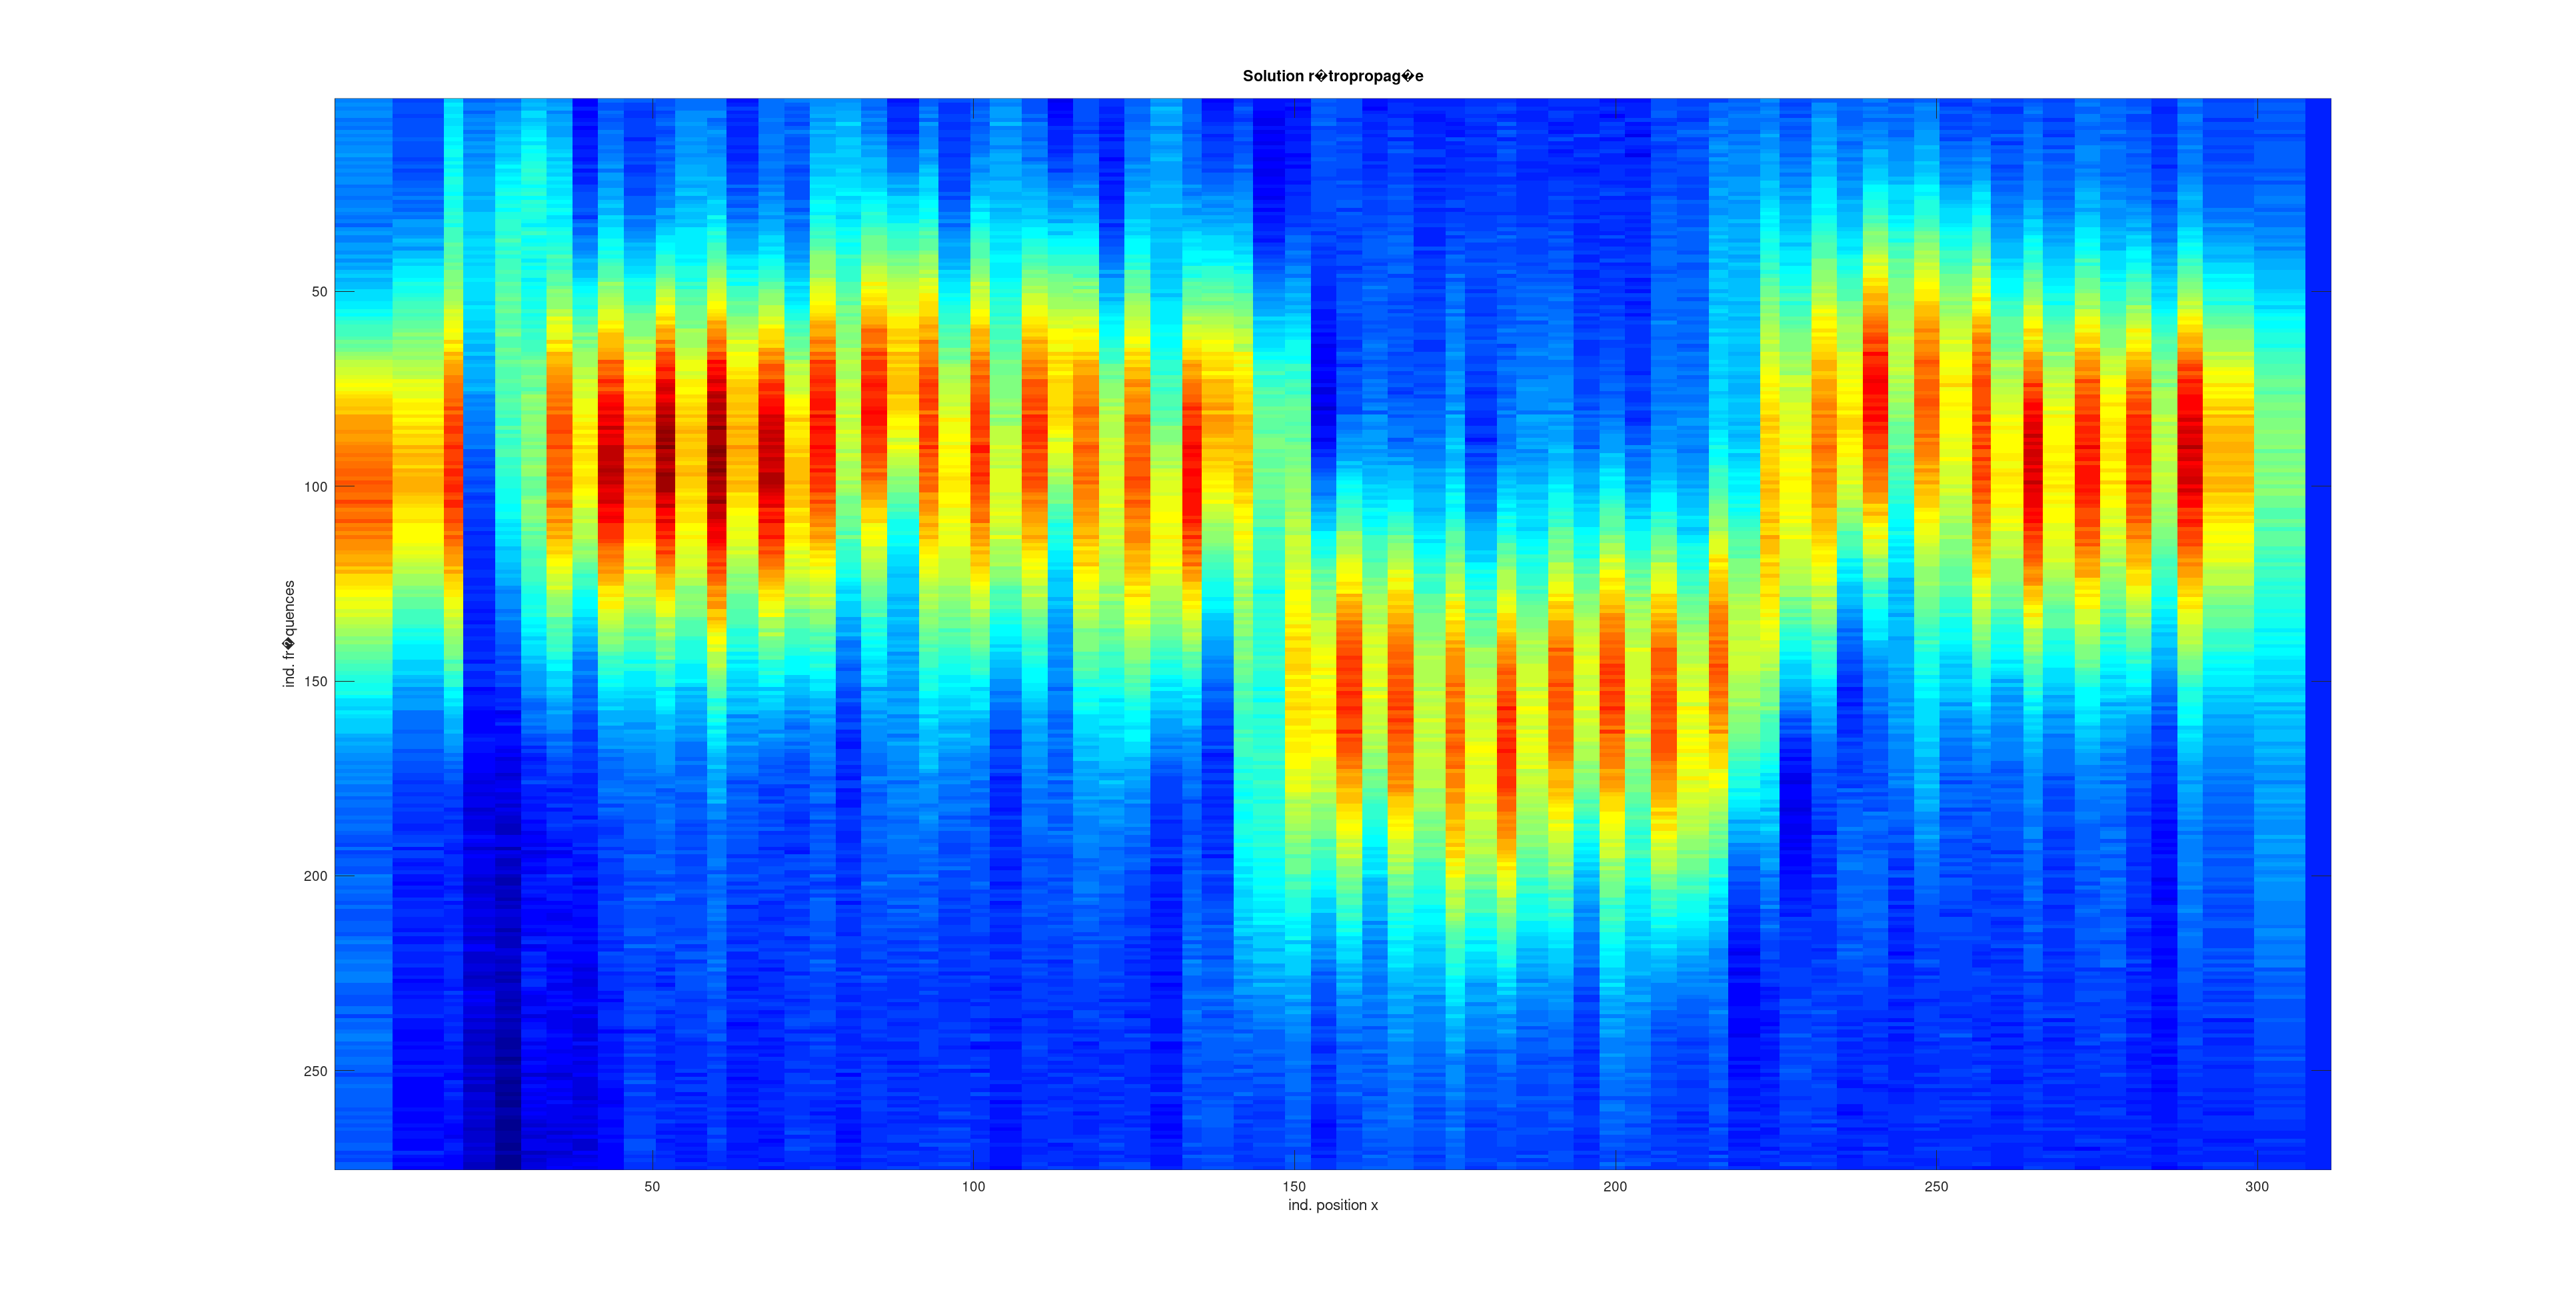
\includegraphics[width=.8\textwidth]{retrop}
    \centering
\end{figure}

Comme on peut le voir sur la figure, on obtient de mauvais résultats causé par le mauvais
conditionnement de la matrice $H$.

Afin d'ontenir une solution plus lisse on introduit un terme de régularisation en nrome 2
pour arriver au critère suivant :

$$ \min \frac{1}{2} \lVert Hx - f \rVert^2 + \frac{\lambda}{2} x^t \Delta_2 x$$

On obtient pour $\lambda = 0.01$ le résultat suivant :

\begin{figure}[H]
    \caption{Solution pour $\lambda = 0.001$}
    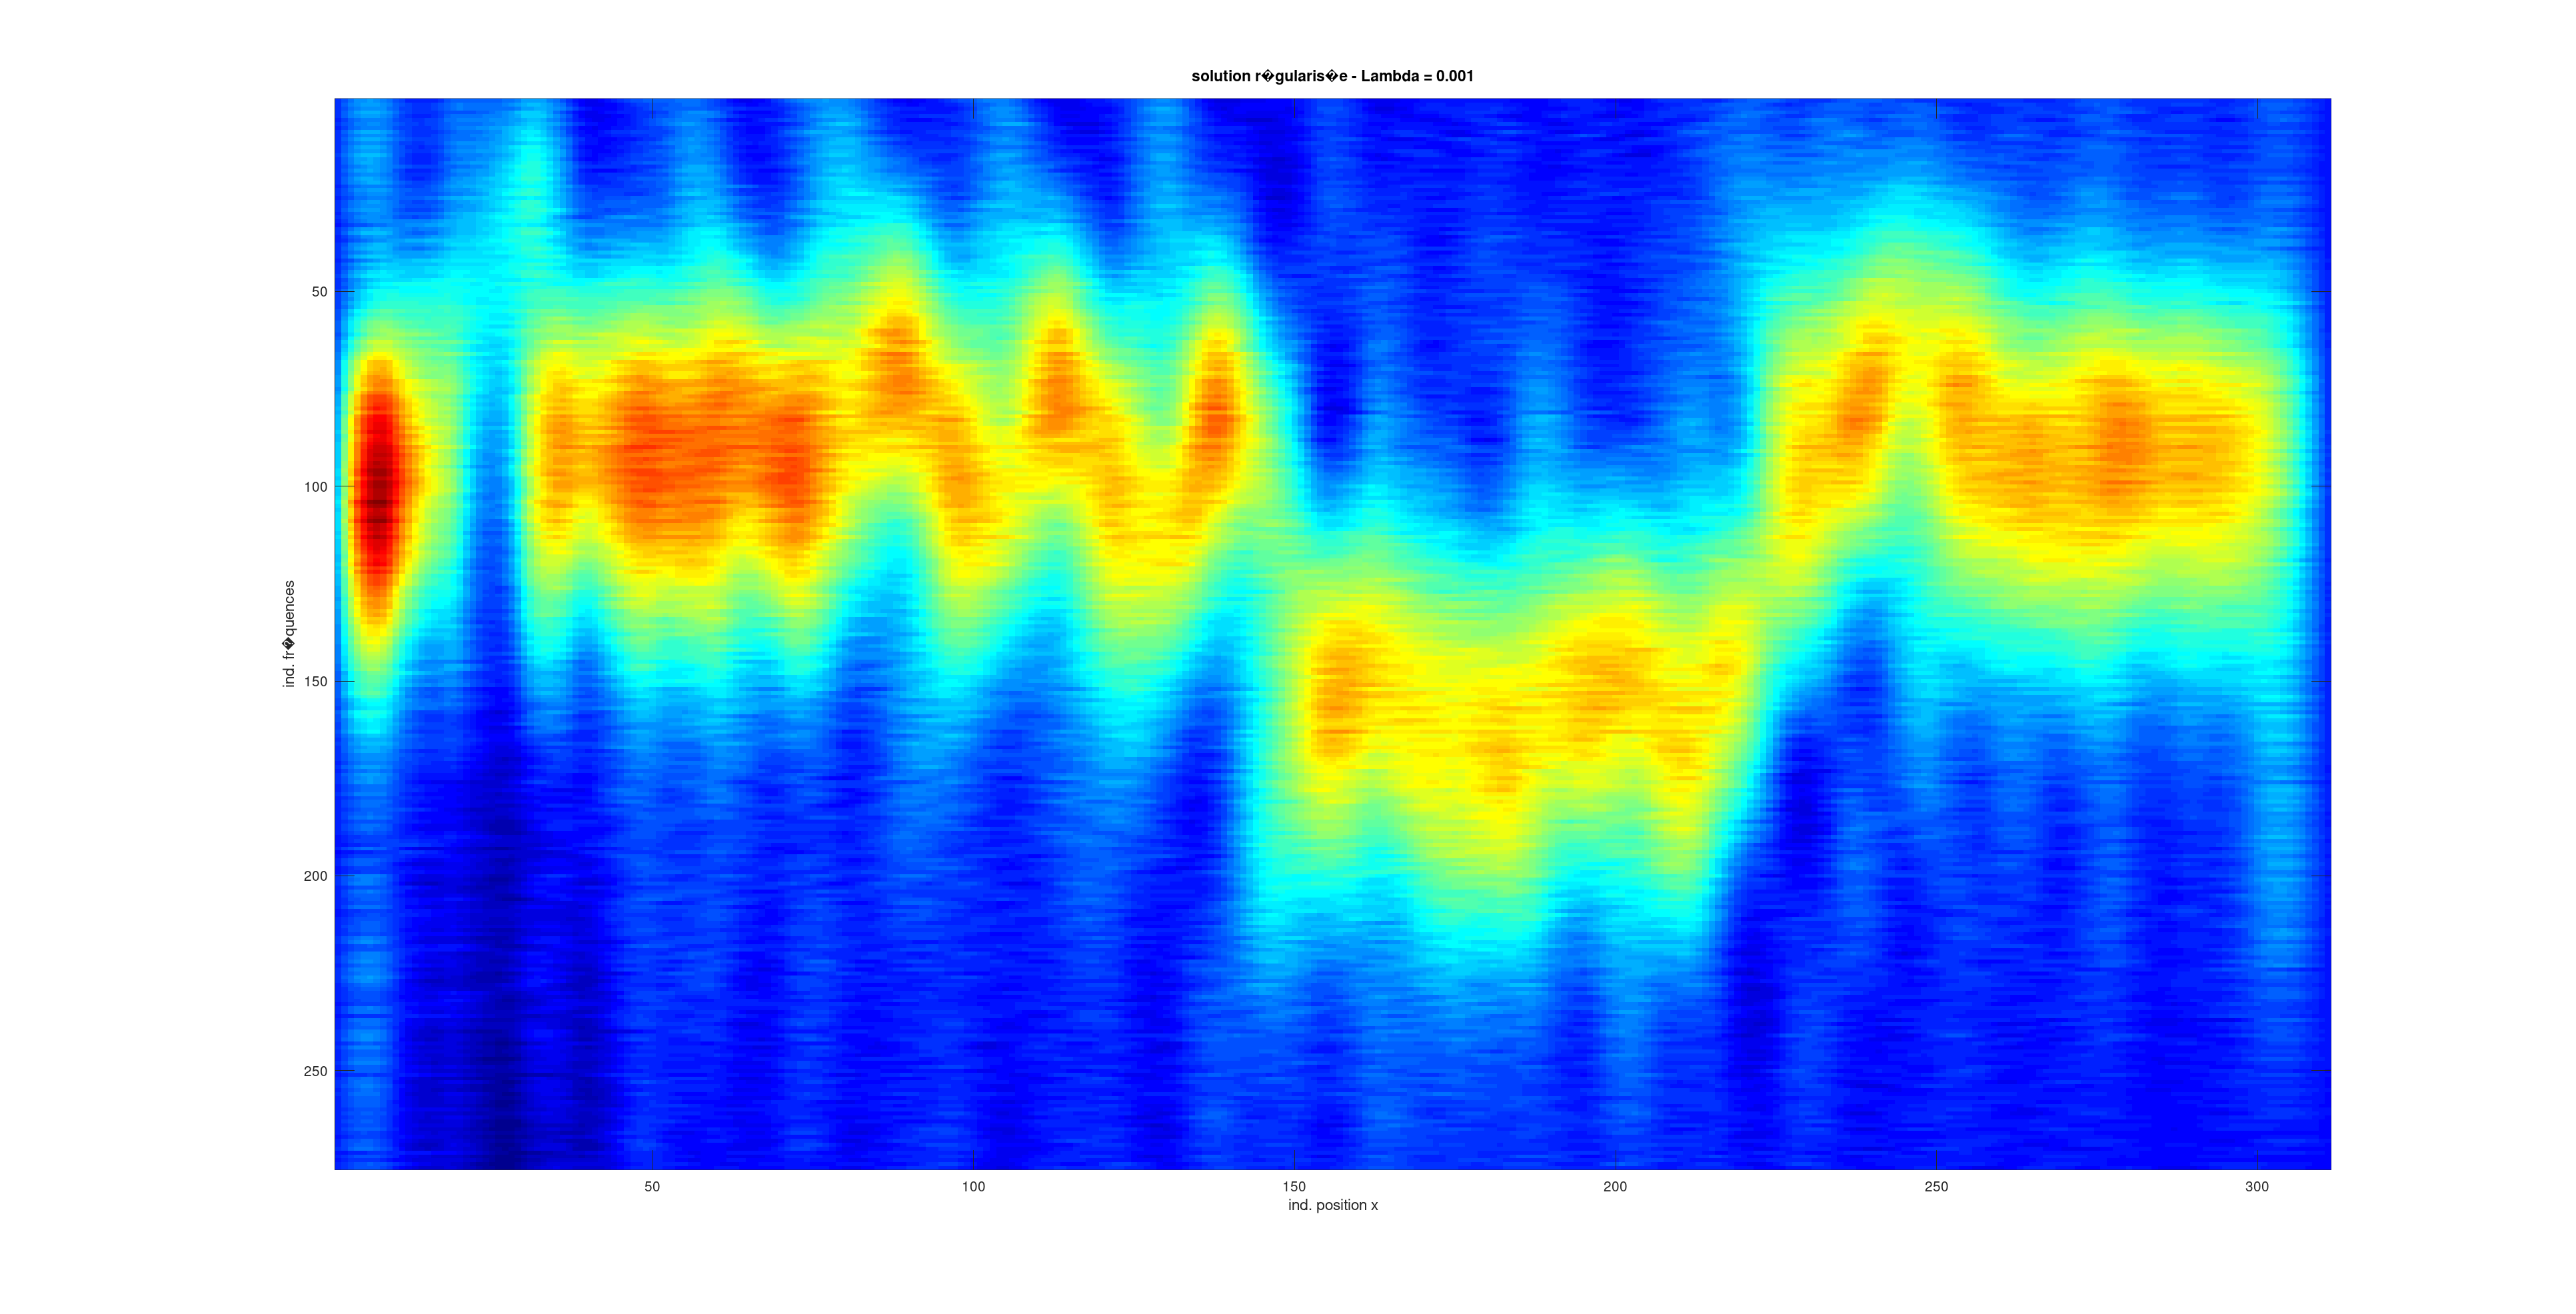
\includegraphics[width=.8\textwidth]{reg1}
    \centering
\end{figure}

\subsection{Influence des paramètres}

Le paramètre sur lequel nous pouvons jouer pour ce problème est $\lambda$, le paramètre
de régularisation.

Ce paramètre est responsable de l'importance accordée à la minimisation du terme
$x^t \Delta_2 x$.

\begin{itemize}
    \item{Pour des valeurs faibles de $\lambda$, on accorde peu d'importance au terme de
        régularisation et on s'approche de la première approche présentée}
    \item{Pour des valeurs élevées de $\lambda$, on accorde beacoup d'importance à la
        régularisation et on obtient une solution trop lisse. On accorde moins d'importance
        aux données mesurées.}
\end{itemize}

Affichons les résultats obtenus pour deux autres valeurs de $\lambda$ :

\begin{figure}[H]
    \caption{Solution pour $\lambda = 0.0001$}
    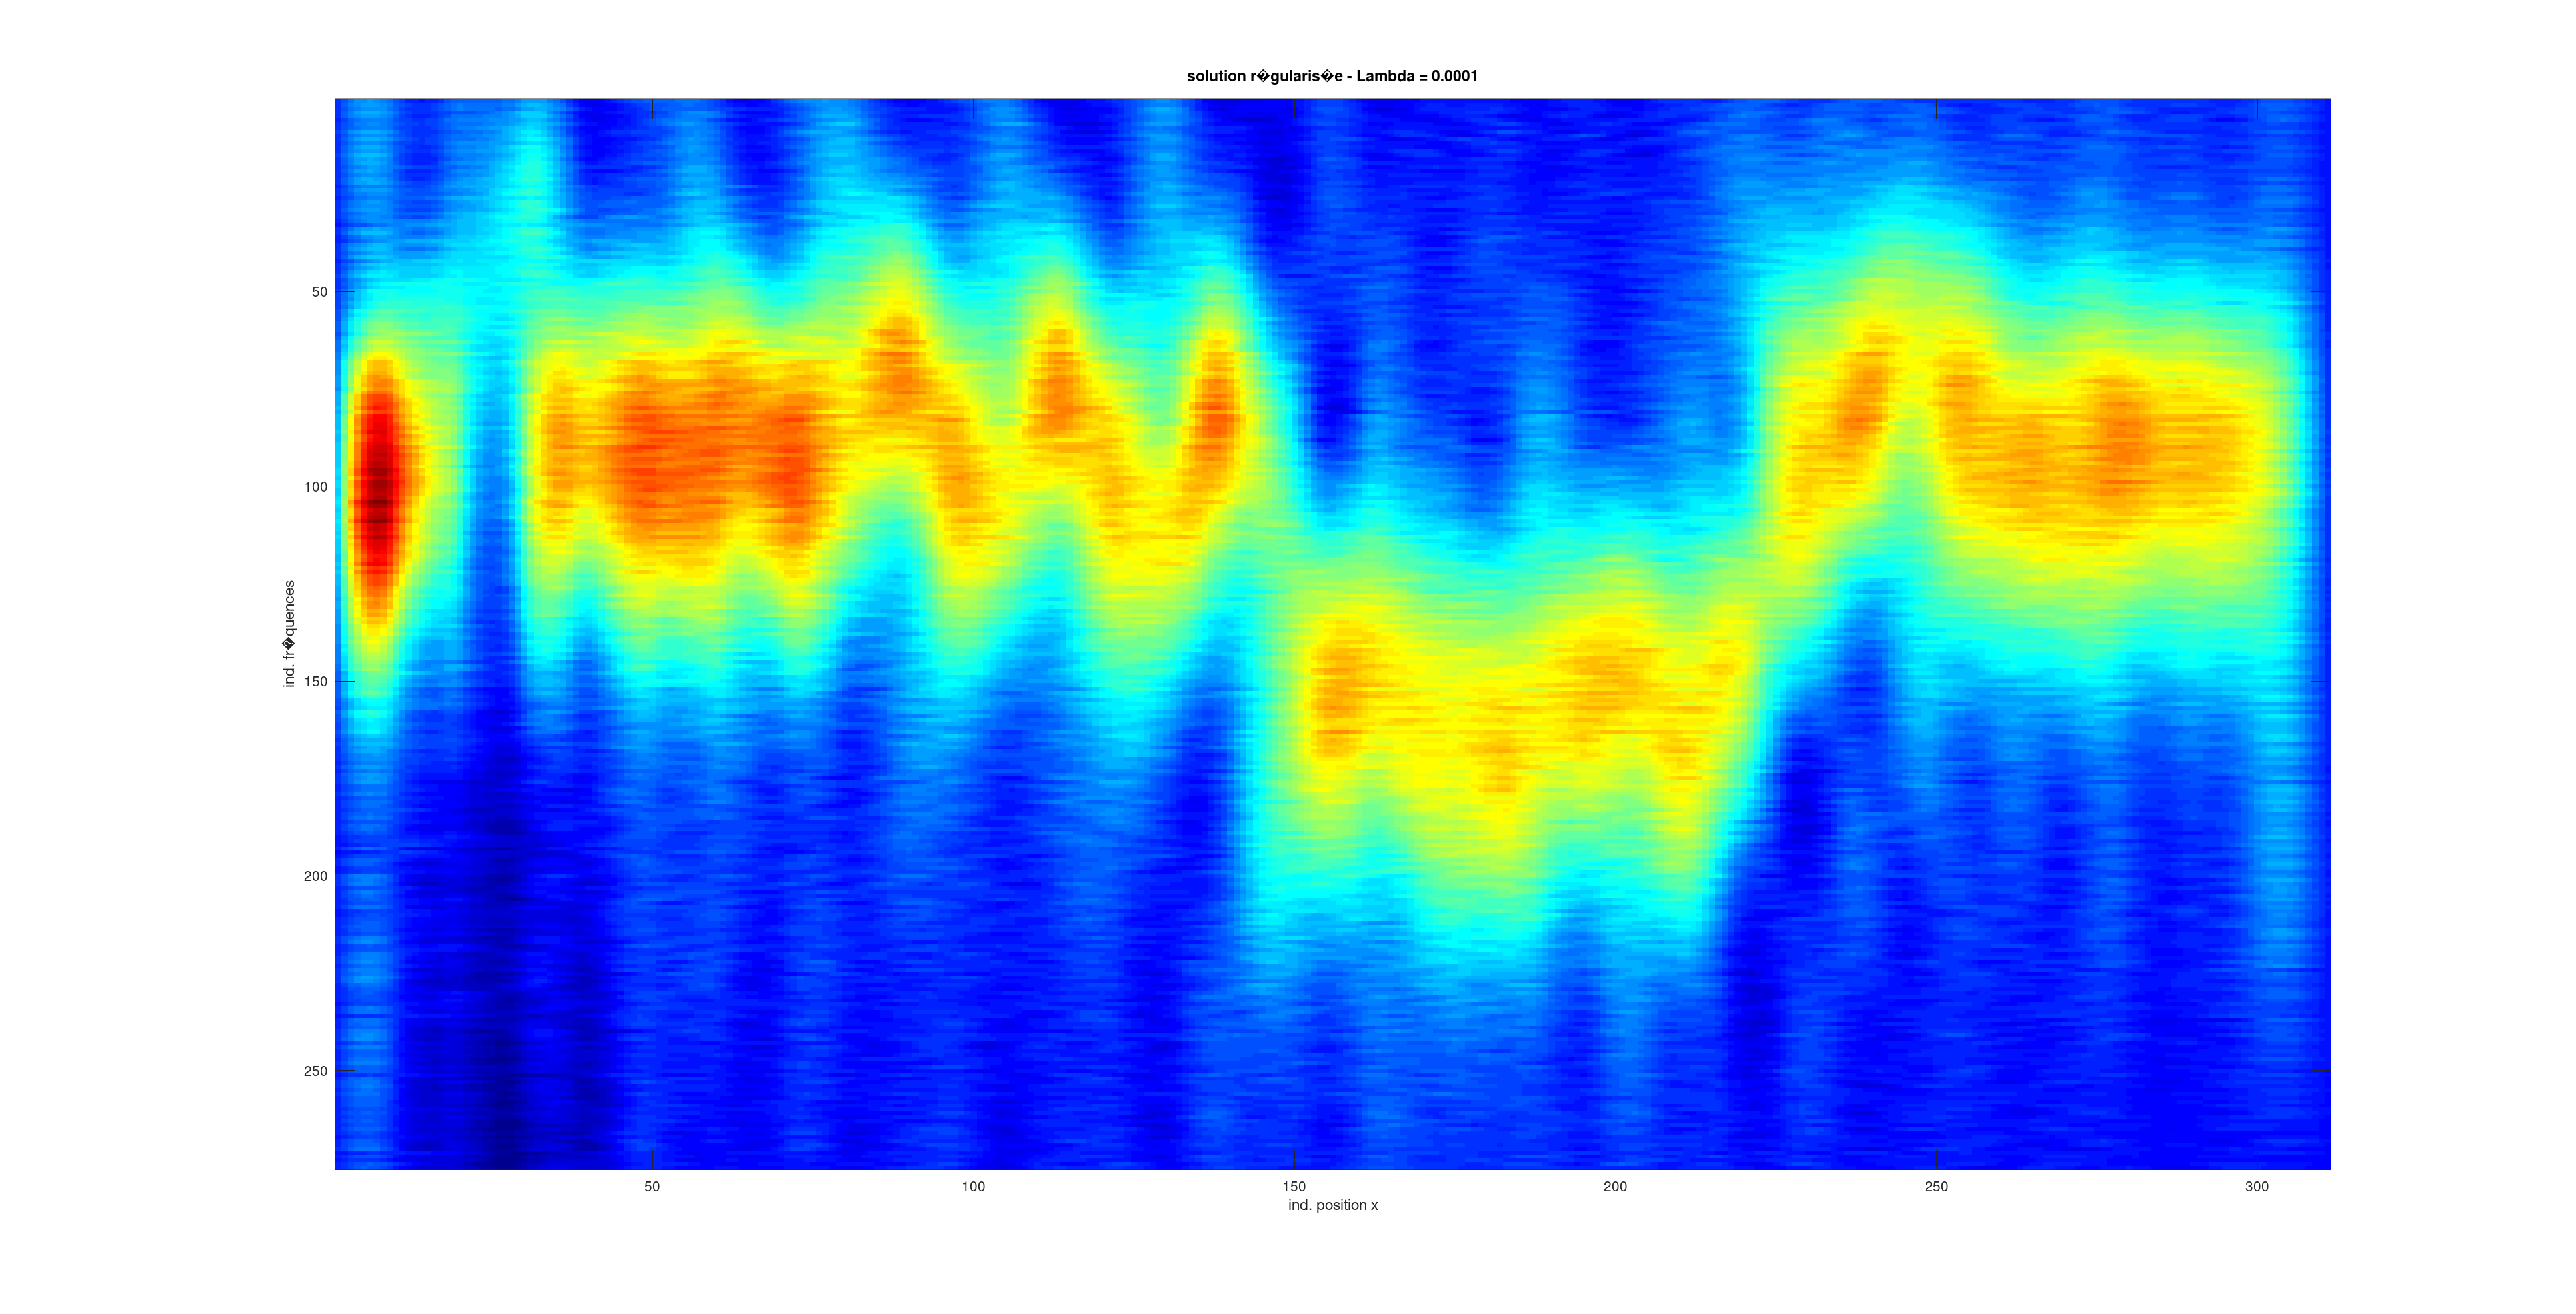
\includegraphics[width=.8\textwidth]{reg2}
    \centering
\end{figure}

\begin{figure}[H]
    \caption{Solution pour $\lambda = 10$}
    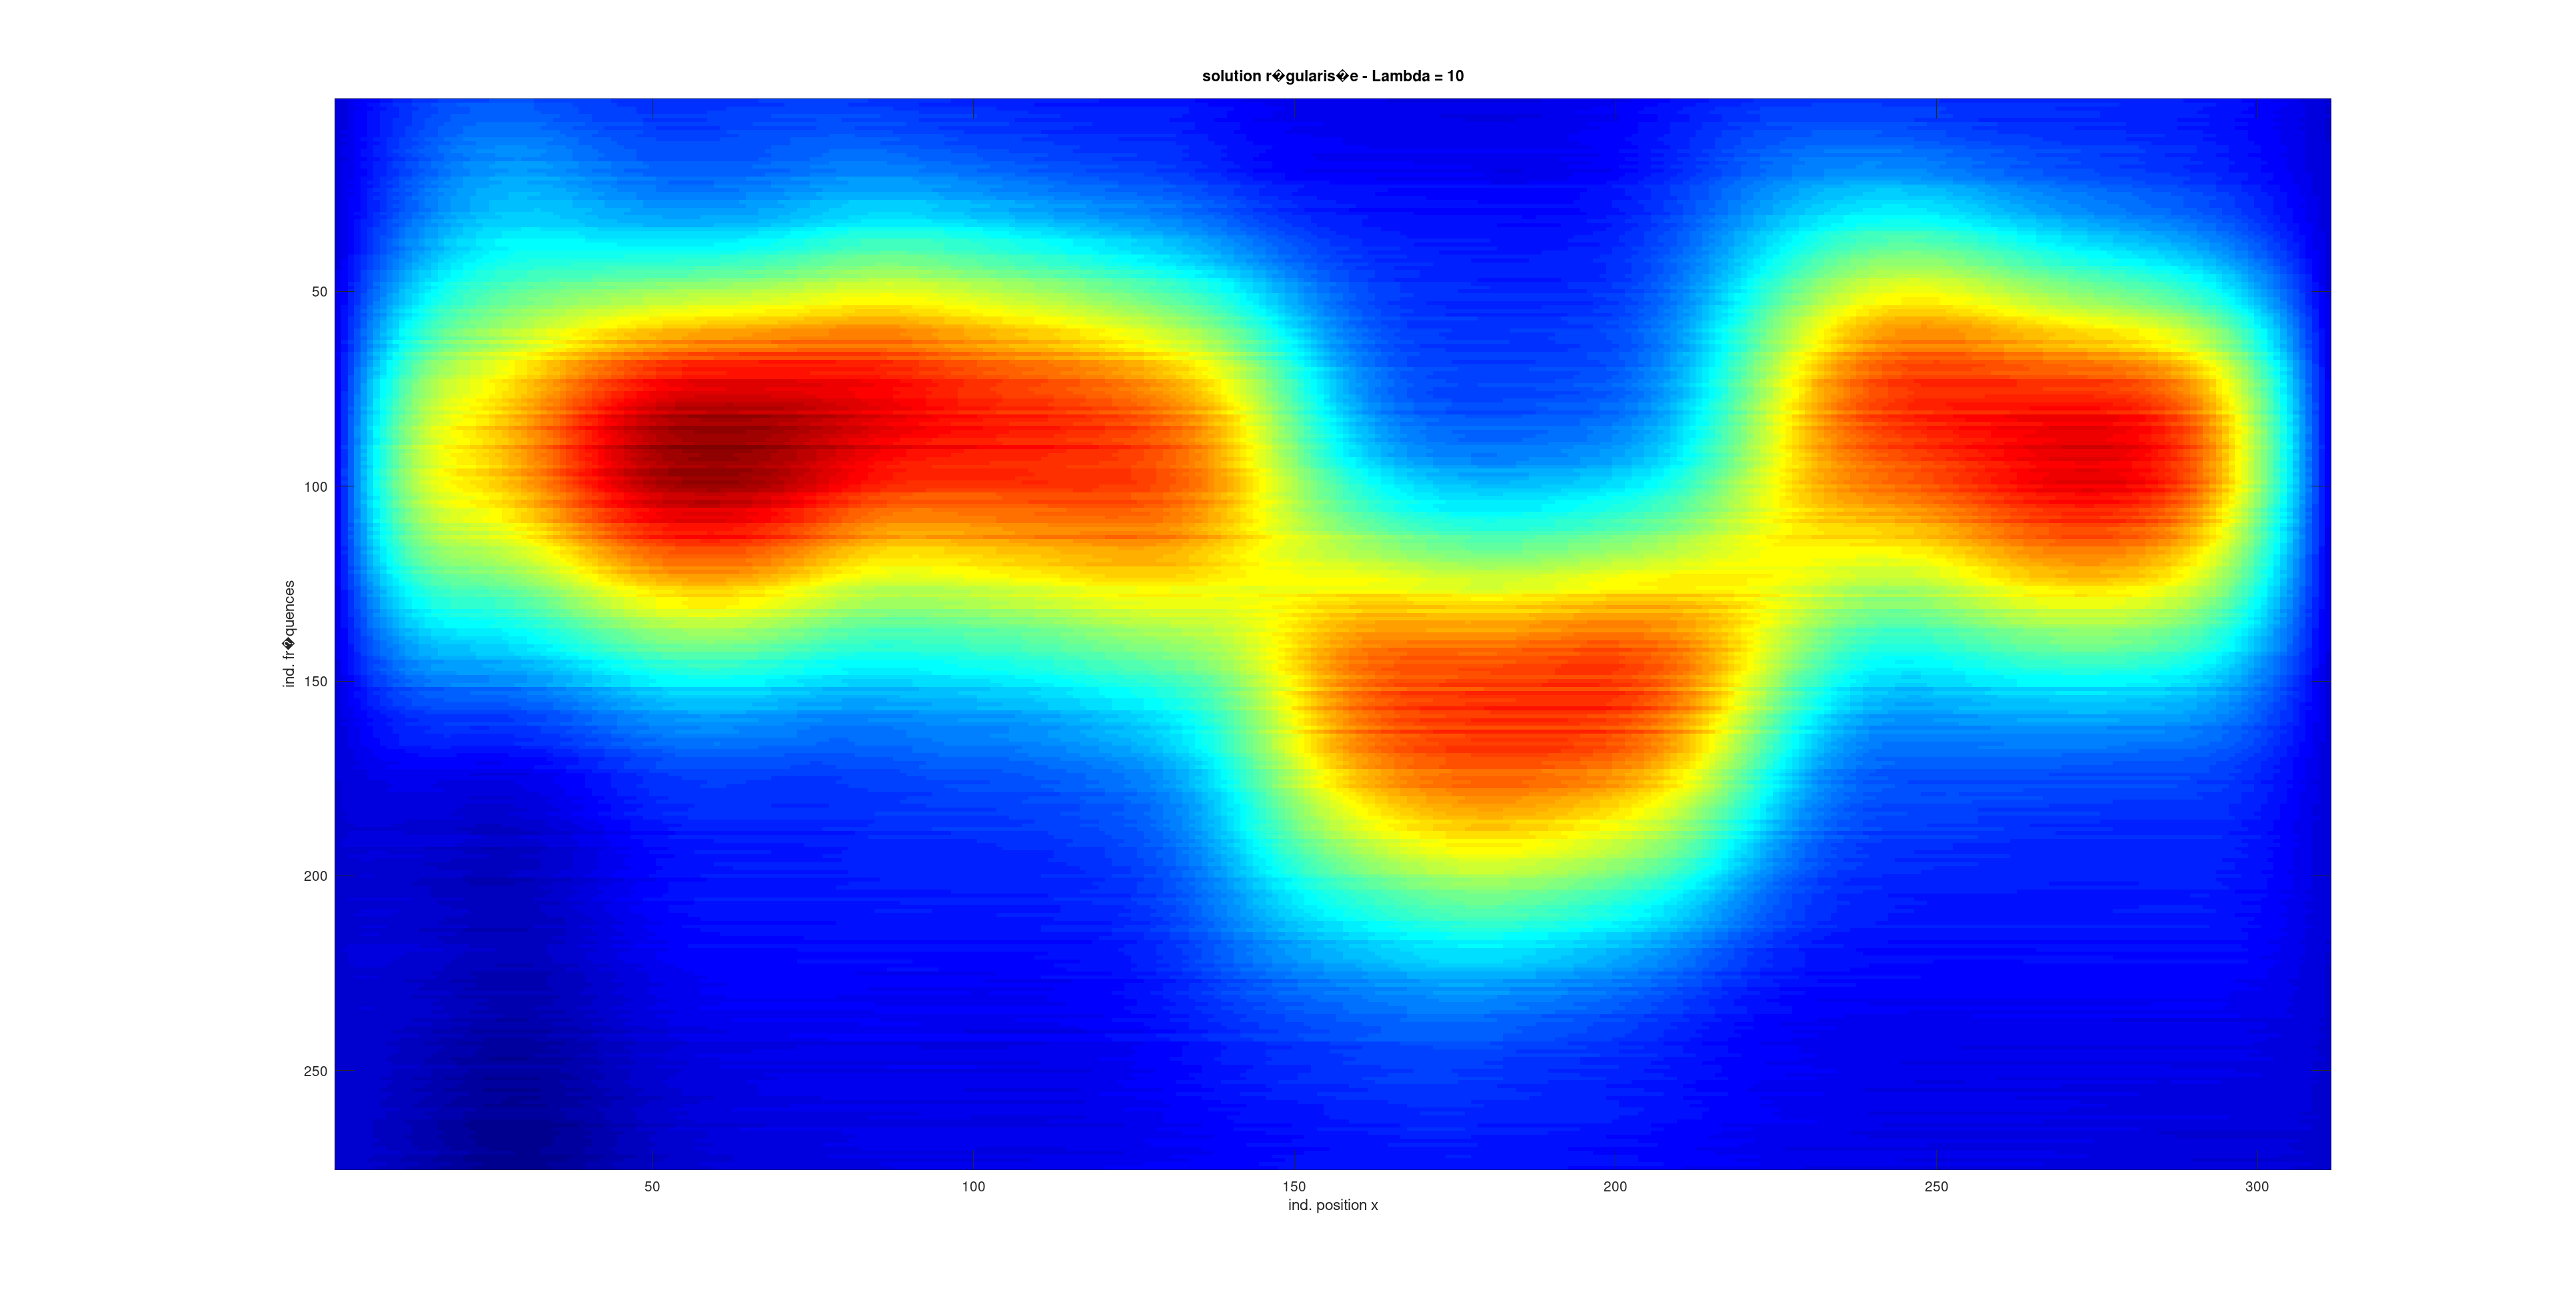
\includegraphics[width=.8\textwidth]{reg3}
    \centering
\end{figure}

On observe bien ce qui a été precisé plus haut.

\begin{itemize}
    \item{Pour $\lambda = 0.001$, on est proche de la solution naïve}
    \item{Pour $\lambda = 10$, on obtient une solution lisse}
\end{itemize}

Il convient alors d'expeimenter avec différentes valeurs de $\lambda$ pour déterminer
laquelel permet d'obtenir les meilleurs résultats en assurant le bon compromis entre
proximité aux données et le lissage.

\pagebreak

\section{Problème inverse de sources à partir de données de contrôle
non-destructif ultrasonore}

\subsection{Le contexte d'application}

L'objectif de cette partie est de réaliser un contrôle non-destructif
de défauts dans des soudures. Pour ce faire, on utilise des signaux
ultrasonores induits par la soudure à inspecter.
On souhaite, à l'aide de ces signaux, détecter des perturbations dues
à ces défauts. Nous disposons alors d'une ondelette de
référence. Elle est réalisée par calibration à l'aide de 4 trous de
1 mm.

On peut donc détecter des défauts similaires à des trous d'un millimètre.
En effet, par déconvolution, on peut retrouver les positions des défauts
(à un décalage près du à la convolution)

\begin{figure}[H]
    \caption{Ondelette et trace à déconvoluer}
    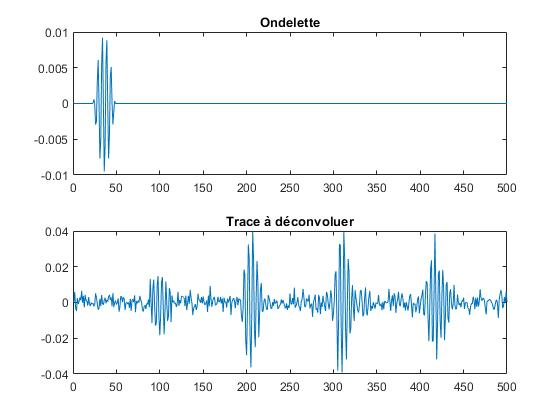
\includegraphics[width=.7\textwidth]{01}
    \centering
\end{figure}

Pour réaliser la déconvolution, on utilise une minimisation de l'erreur
quadratique moyenne. En revanche, sans information à priori sur la
réflectivité, on obtient des résultats de mauvaise qualité. On utilise
alors une régularisation :

$$ J(r) = \lVert z - Hr \rVert^2 + \lambda \Phi(r) $$

On obtient donc une nette amélioration par rapport à la trace à déconvoluer mais,
le défaut apparait avec un double pic :

\begin{figure}[H]
    \caption{Identification Réelle}
    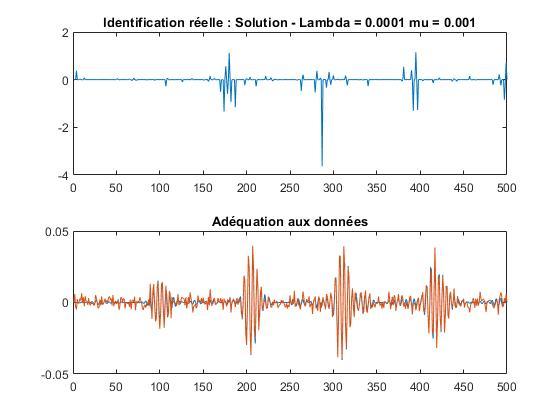
\includegraphics[width=.7\textwidth]{02}
    \centering
\end{figure}

Pour tenir compte de la possible déformation en phase de l'ondelette,
on a recours à la transformée de Hilbert de l'ondelette $h$. On obtient
alors un nouveau modèle de convolution ainsi qu'un nouveau critère
à minimiser. On obtient le nouveau critère :

$$ J(r,s) \lVert z - Hr - Gs \rVert^2 + \lambda \Phi(r,s) $$

Et le résultat suivant :

\begin{figure}[H]
    \caption{Identification Complexe}
    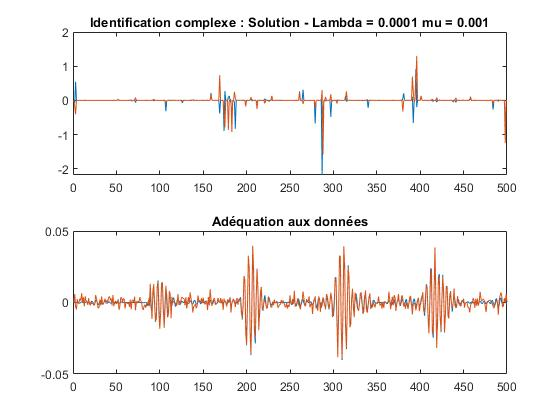
\includegraphics[width=.7\textwidth]{03}
    \centering
\end{figure}

On peut également observer le module des deux solutions sur le graphique
ci-dessous :

\begin{figure}[H]
    \caption{Comparaison des deux approches}
    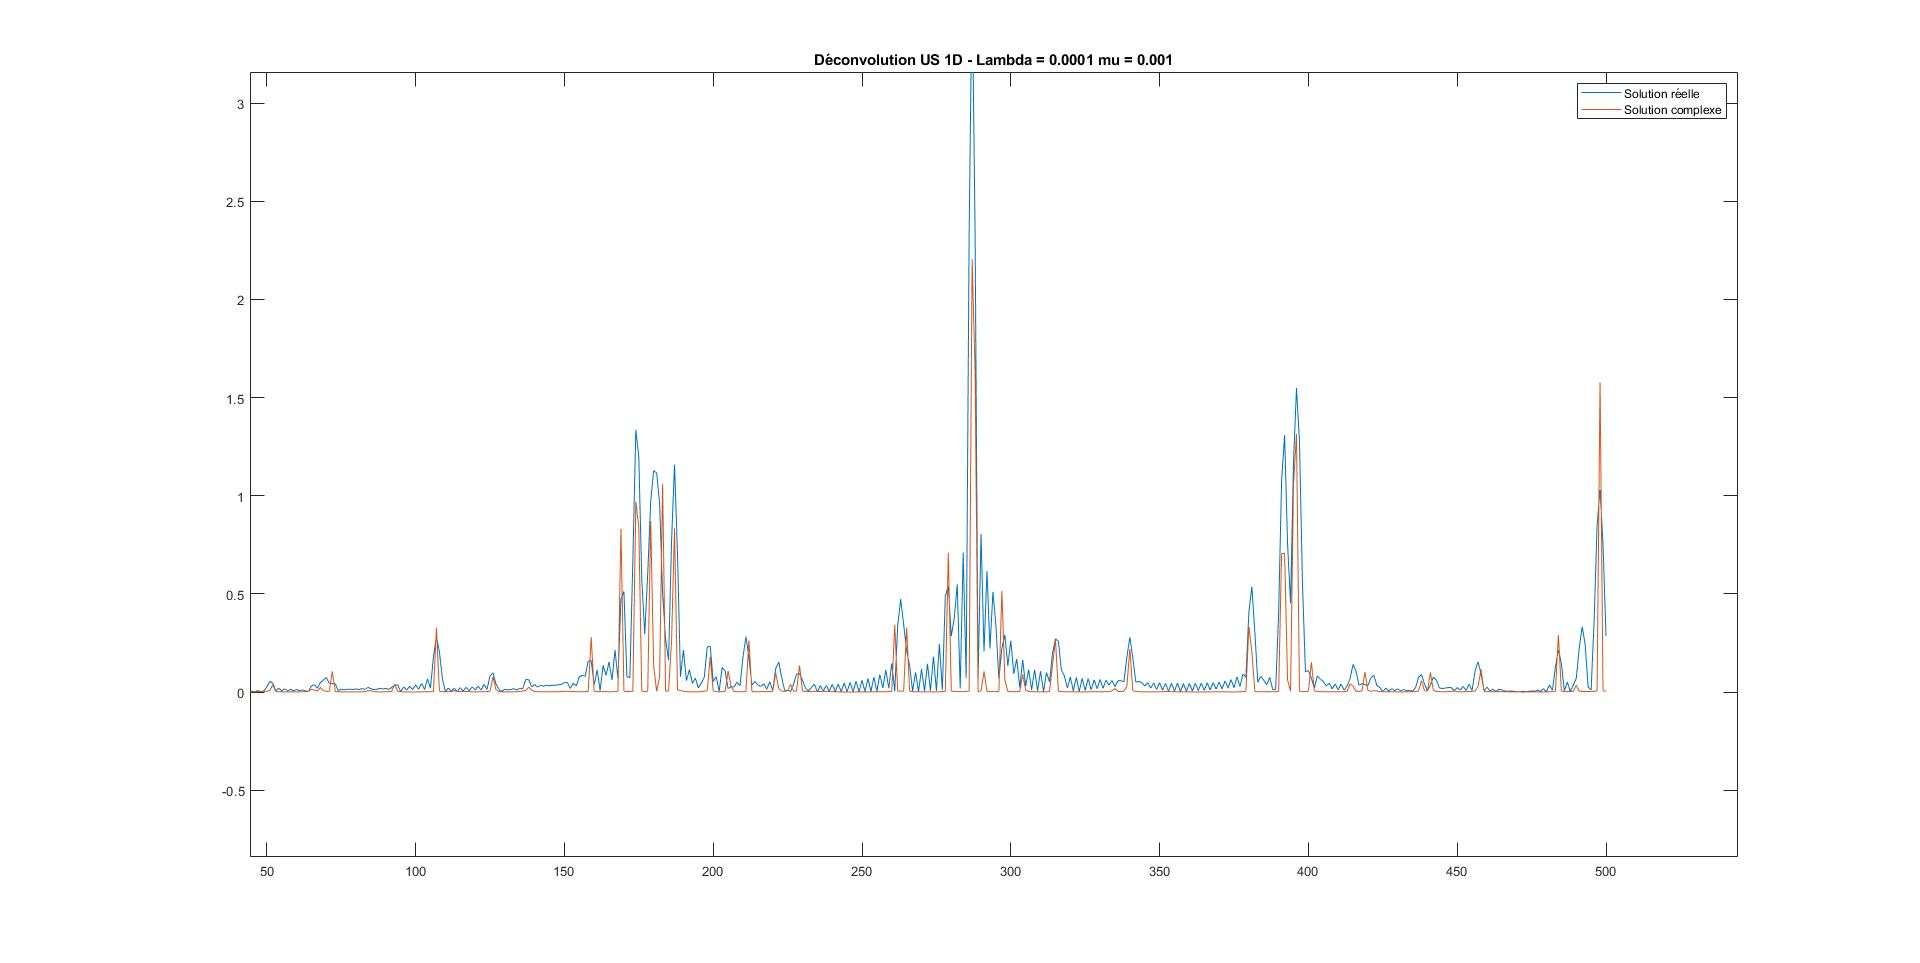
\includegraphics[width=.7\textwidth]{04}
    \centering
\end{figure}

\subsection{Influence des paramètres}

On constate sur la figure ci-dessus que le choix des paramètres n'est
clairement pas optimal.

En effet, pour ce problème nous disposons de deux paramètres, $\lambda$
et $\mu$ :

\begin{itemize}
    \item{Le paramètre $\mu$ permet de s'assurer de l'existence de la solution et
        doit être non nul. Plus il est proche de 0, plus la solution
        est optimale. En revanche, l'optimisation sera plus complexe. On
        choisit alors une valeur $\mu = 10^{-2}$ pour obtenir un bon
        compromis.}
    \item{Le paramètre $\lambda$ correspond au paramètre de régularisation.
        Il contrôle le poids du terme de régularisation.}
\end{itemize}

Dans la partie précedente, nous avons choisi une valeur très faible pour
le paramètre de régularisation : $\lambda = 10^{-4}$. On obtenait donc
uen solution non optimale. En effet pour des valeurs faibles de $\lambda$,
la régularisation aura un effet négligeable tandis qu'au contraire,
pour des valeurs trop importantes de $\lambda$, on surrégularise.

On constante alors que pour une valeur $\lambda = 10^{-3}$, on obtient
les meilleurs résultats.

Pour la solution réelle :

\begin{figure}[H]
    \caption{Identification réelle}
    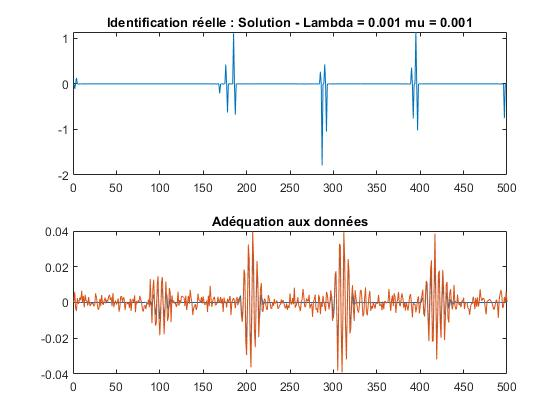
\includegraphics[width=.7\textwidth]{02-opti}
    \centering
\end{figure}

Et pour la solution complexe :

\begin{figure}[H]
    \caption{Identification complexe}
    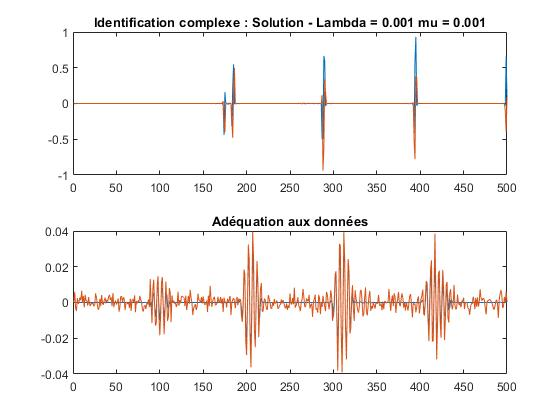
\includegraphics[width=.7\textwidth]{03-opti}
    \centering
\end{figure}

Et enfin, pour les modules :

\begin{figure}[H]
    \caption{Comparaison des deux approches}
    \label{fig:4opti}
    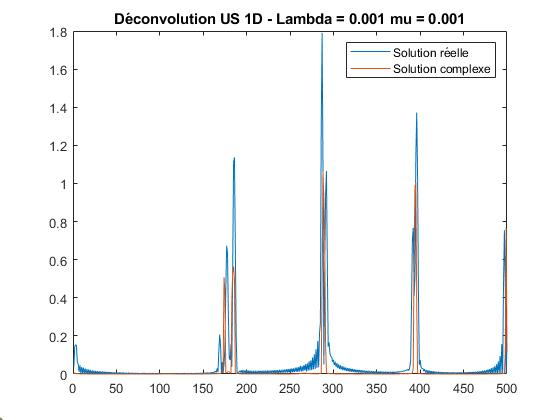
\includegraphics[width=.7\textwidth]{04-opti}
    \centering
\end{figure}

Pour des valeurs de $\lambda$, plus élevées, les pics sont trop épais
et on perd donc en résolution.

\textbf{Remarque} : On peut observer sur la figure \ref{4opti} que la solution complexe
est bien plus intéressante que la solution réelle. En effet, on obtient
bien un seul pic par défaut. Cependant, on remarque que pour le premier
défaut, la solution complexe nous donne aussi 2 pics. Il s'agit en fait d'un défaut
différent qui ne correspond pas à un trou mais à un défaut de surface et qui
nécessite alors une autre ondelette afin d'être correctement detecté.

\end{document}
